\documentclass[sigconf]{acmart}

\def\BibTeX{{\rm B\kern-.05em{\sc i\kern-.025em b}\kern-.08emT\kern-.1667em\lower.7ex\hbox{E}\kern-.125emX}}
\usepackage{subfigure}
\usepackage{algorithm}
%\usepackage{algorithmic}
\usepackage{algpseudocode}
\usepackage{amsmath}
\usepackage{graphics}
\usepackage{epsfig}
\usepackage{multirow}
\usepackage{graphicx}
\usepackage{subfigure}
\usepackage{array}

\begin{document}

\title{Approximate Code: A Cost-Effective Erasure Coding Framework for Tiered Video Storage in Cloud Systems}

\author{Huayi Jin, Chentao Wu, Xin Xie, Jie Li, Minyi Guo, Hao Lin, Jianfeng Zhang}
%\email{keplar_gd@sjtu.edu.cn}
\affiliation{%
  \institution{Shanghai Jiao Tong University}
}


\author{Hao Lin, Jianfeng Zhang}
\authornotemark[1]
\affiliation{%
  \institution{The Alibaba Group}
}

\begin{abstract}
Nowadays massive video data is stored in cloud storage systems, which is generated by various applications such as autonomous driving, news media, security monitoring, etc. Meanwhile, erasure coding is a popular technique in cloud storage to provide both high reliability with low monetary cost, where triple disk failure tolerant arrays (3DFTs) is a typical choice. Therefore, how to minimize the storage cost of video data in 3DFTs is challenge for cloud storage systems. Although there are several solutions like approximate storage technique for storage devices, it cannot guarantee low storage cost and high data reliability in storage systems concurrently.

To address this problem, in this paper, we propose Approximate Code, which is an erasure coding framework for tiered video storage in cloud systems. The key idea of Approximate Code is distinguishing the important data and unimportant data in videos with different capabilities of fault tolerance. On one hand, for important data, Approximate Code provides triple parities to provide high reliability. On the other hand, single/double parities are applied for unimportant data, which can save the storage cost and accelerate the recovery process. To demonstrate the effectiveness of Approximate Code, we conduct several experiments in Hadoop systems. The results show that, compared to traditional 3DFTs using various erasure codes such as RS, STAR and TIP-Code, Approximate Code reduces the number of parities by up to 55\%, saves the storage cost by up to 20.8\%, increase the recovery speed by up to 1.25X when single disk fails, and can reconstruct the whole video data via fuzzification when triple disks fail.
\end{abstract}

\ccsdesc[500]{Information systems~Distributed storage}
\ccsdesc[500]{Computer systems organization~Dependable and fault-tolerant systems and networks}

\keywords{Erasure Codes, Approximate Storage, Multimedia, Cloud Storage}
\maketitle

\section{Introduction}
For typical cloud storage systems such as Windows Azure \cite{calder2011windows} and Amazon AWS \cite{bermudez2013exploring}, erasure coding is a popular technique to provide both high reliability and low monetary cost \cite{EVENODD, RDP, BlaumRoth, XCode, CRS, TripleStar, TPtech, RSL}, where triple disk failure fault tolerant arrays (3DFTs) are widely used. Typical erasure codes can be divided into two categories, RS-based Codes \cite{RS} \cite{LRC} and XOR-based codes \cite{EVENODD, hcode, STAR, tip}. RS-based codes are encoded according the Galois Field Computation in Reed Solomon Code \cite{RS}, which allow flexible configuration and have a little higher computation cost. XOR-based codes simplify the computation, but the scalability is a significant issue in previous literatures.

With the increasing demand on higher resolution and frame rate for video data, massive storage devices are highly desired in cloud storage systems, which makes data centers much bigger.
Therefore, in this paper, we set out to answer the following question:

\textbf{In a cloud storage system, how to efficiently store tremendous video data in 3DFTs?}

To reduce the storage cost in cloud storage systems, a feasible solution is approximate storage. Approximate storage exposes unimportant data to errors, saving the overhead of redundant backups \cite{niklaus2018context, sampson2014approximate} , thus the data reliability cannot be guaranteed.
Another solution is using disk arrays like RAID-5 or RAID-6 \cite{RAID}, but the capability of fault tolerance are sacrificed.
Data compression\footnote{Typically, video coding (e.g., H.264 \cite{wiegand2003overview}) is a special type of data compression.} is also a common strategy for reducing storage overhead \cite{ziv1977universal, ziv1978compression, deutsch1996deflate}.
\textcolor{red}{However, the compression and decompression processes result in a large amount of computational overhead, which decreases their efficiency in frequent failure scenarios like cloud.}
Therefore, existing solutions cannot provide low storage cost and high reliability simultaneously.

To address the above problem, in this paper, we propose Approximate Code, which is an erasure coding framework to provide comprehensive solution for video data storage in cloud systems. The key idea of Approximate Code is treating the important/unimportant data in different ways. For important data, we add additional parities to provide high capability of fault tolerance. On the other hand, the unimportant data are encoded with a minimum number of parities, which only supply the basic requirement of the recovery. When triple disks fail, the lost data can be reconstructed via a fuzzy manner.

We have the following contributions of this work,
\begin{enumerate}
\item We propose Approximate Code, which a cost-effective framework to store video data in cloud storage systems.
\item Approximate Code can be implemented by combining various erasure codes in 3DFTs, such as RS, STAR Code, TIP-Code, etc.
\item We conduct several quantitative analysis, simulations and experiments according to different layouts of various erasure codes, and the results show that Approximate Code achieves lower storage cost and faster data recovery when single disk fails.
\end{enumerate}

The rest of the paper is organized as follows. In Section \ref{RelatedWork}, we introduce related work and our motivation.
In Section \ref{ApCode}, the design of Approximate Code and its encoding and decoding process will be illustrated in detail.
%Section \ref{Implementation} introduce the implementation of our design, and section \ref{ap-recovery} analysis the performance of approximate video storage.
The evaluation is presented in Section \ref{evaluation} and the conclusion of our work is in Section \ref{Conclusion}.

\section{Related Work and Our Motivation}\label{RelatedWork}
In this section, we introduce the background of video storage, existing solutions to reduce storage cost and the motivation of this paper.
To facilitate the discussion, we summarize the symbols used in this paper in Table \ref{parameter}.

\begin{table}[]\footnotesize
\caption{The symbols used in this paper.}\label{parameter}
\centering
\begin{tabular}{|p{0.7cm}<{\centering}|p{6.5cm}|}
\hline
Symbols & \multicolumn{1}{c|}{Description} \\ \hline \hline
$k$ & the number of data nodes in a local stripe \\ \hline
$r$ & the number of local parity nodes in a local stripe \\ \hline
$n$ & the number of all data and parity nodes in a local stripe. ($n=k+r$) \\ \hline
$h$ & the number of local stripes to construct a global stripe \\ \hline
$g$ & the number of global parity nodes \\ \hline
$N$ & total number of all nodes ($N=(k+r)h+g$) \\ \hline
$E_{i,j}$ & the element at the $i$-th row and $j$-th column \\ \hline
$D_i$ & a data node \\ \hline
$P_{I}$ & the mathematical expectation of important data being recoverable under faults that exceed fault tolerance \\ \hline
$P_{U}$ & the mathematical expectation of unimportant data being recoverable under faults that exceed fault tolerance \\ \hline
$\oplus$ & the XOR operation symbol \\ \hline
$\binom{n}{k}$ & The number of $k$-combinations from $n$ elements\\ \hline
LP & local parity nodes \\ \hline
GP & global parity nodes \\ \hline
ID & important data in a video file \\ \hline
UD & unimportant data in a video file \\ \hline
\end{tabular}
\end{table}


\subsection{Basis of Video Storage}\label{video storage}
For normal HD (resolution 1280$\times$720, 8-bit, 30 fps) video, the amount of raw video data in 1 minute is 4.63 GB, so video data is usually encoded by lossy compression algorithms before storage.

\subsubsection{Video coding}
H.264 \cite{wiegand2003overview} is one of the advanced algorithms. This coding technique is widely used on platforms such as YouTube because it has higher compression ratio and lower complexity than its predecessor. For a normal HD video file metioned as above, H.264 can reduce its size by about 10 times, only 443.27MB.

H.264 classifies all frames into three different categories:
\begin{enumerate}
    \item I frame: A frame that does not depend on other frame data, which means it can be decoded independently of other frames.
    \item P frame: A frame holds the changes compared to the previous frame, thus saving much space by leaving out redundant information.
    \item B frame: A frame saves more space by utilizing the data of both the preceding and following frame.
\end{enumerate}
A group of pictures (GOP) consists of one I frame followed by a number of consecutive P and B frames that are independent of the frames in other GOPs to prevent bit error spread, as shown in Figure \ref{H264-IPB}.
%In other words, a P or B frame can only reference the ones inside the GOP which it belongs to, as shown in Figure \ref{H264-IPB}.
Therefore, within each GOP, the I frame has the highest importance because other frames rely on it for recovery; the importance of the P frame is second, and the B frame has the least importance. Based on this feature, a special program can be designed to distinguish the importance of video frames.

\begin{figure}[ht]
\centering
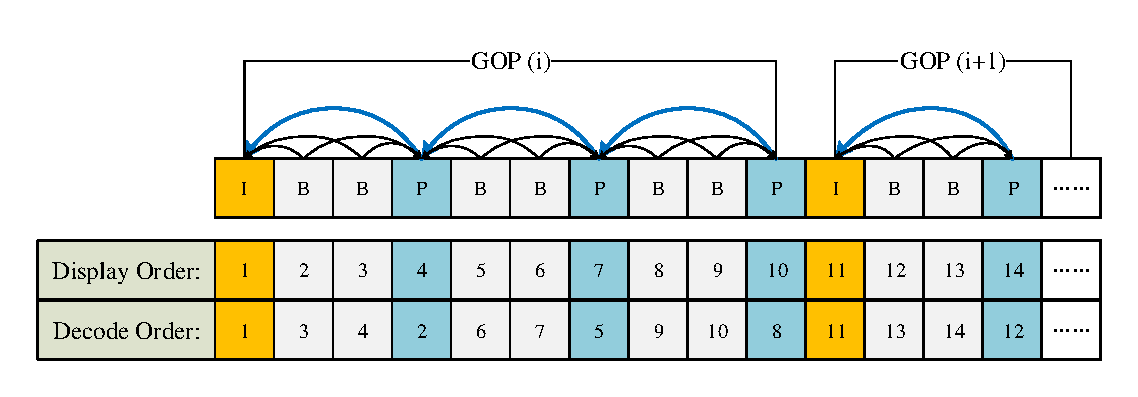
\includegraphics[width=0.45\textwidth]{photo/H264_IPB.pdf}
\caption{A sample of GOPs in H.264}
\label{H264-IPB}
\end{figure}

\subsubsection{Video Frame Recovery}
In the circumstance of video approximate storage, it's common to lose some frames and leave the video incomplete. However, the lost frames can still be recoverable with the benefit of nowadays powerful deep learning techniques. One of them is named video frame interpolation \cite{meyer2015phase, niklaus2018context}.

Video frame interpolation is one of the basic video processing techniques, an attempt to synthetically produce one or more intermediate video frames from existing ones. This is a technique that can model natural motion within a video, and generate frames according to the model.

In deep learning methods, optical changes between the frames are trained in a supervised setup mapping two frames to their ground truth optical flow. Among all these, a multi-scale network\cite{van2017frame} based on recent advances in spatial transformers and composite perceptual losses has so far produced the new state-of-the-art results in terms of Peak Signal to Noise Ratio (PSNR), and so has a context-aware Synthesis approach\cite{niklaus2018context} in terms of Middlebury benchmark.

\subsection{Existing Erasure Codes}\label{existEC}

Reliability is a critical issue since disk failures are typical in storage systems. To improve the reliability of storage systems, several RAID forms (e.g., RAID-5, RAID-6, 3DFTs) and erasure codes are proposed by researchers.  Traditional erasure codes can be categorized into two classes, Maximum Distance Separable (MDS) codes and non-MDS codes. MDS codes aim to offer data protection with optimal storage efficiency. On the other hand, non-MDS codes improve the performance or reliability by consuming extra storage space.

In the past two decades, several famous erasure codes are proposed for double Disk Failure Tolerant arrays (2DFTs or RAID-6), such as EVENODD code \cite{EVENODD}, RDP code \cite{RDP}, Blaum-Roth code\cite{BlaumRoth}, X-code \cite{XCode}, Liberation code \cite{Liberation}, Liber8tion code \cite{Liber8tion}, Cyclic \cite {Cyclic} code, B-Code \cite{BCode}, Code-M \cite{Code-M}, H-code \cite{hcode}, P-code \cite{PCode} and HVcode \cite{HVCode}, etc.

In Triple Disks Failure Tolerant Arrays (3DFTs), typical MDS codes include Reed-Solomon codes \cite{RS}, Cauchy-RS codes \cite{CRS}, STAR code \cite{STAR}, Triple-Star code \cite{TripleStar}, Triple-Parity code \cite{TPtech}, HDD1 code \cite{HDD}, RSL-code \cite{RSL}, RL-code \cite{RL}, and so on. Typical non-MDS codes contain WEAVER codes \cite{WEAVER}, HoVercodes \cite{HoVer}, T-code \cite{TCode}, HDD2 code \cite{HDD}, Pyramid codes \cite{Pyramid}, Local Reconstruction Codes \cite{LRC}, Locally Repairable Codes \cite{XORing}, etc.
In the following we mainly introduce the classic erasure codes used in this paper.

Reed Solomon Code \cite{RS} (RS code) is a classic MDS code. The encoding and decoding operations of RS code are based on Galois Field (GF), leading to high scalability as well as high computational complexity. All the parities of RS code are horizontal as shown in Figure \ref{fig-RS-1}.

\textcolor{red}{Need to update}
Local Construction Code (LRC) \cite{LRC} divides the data nodes into multiple local groups, each with a local parity node, and the global parity is calculated by all data nodes. Therefore, when a single node is corrupted, data can be recovered by local parity without requiring access to all nodes.
LRC reduce the bandwidth and I/Os required for repair reads at the expense of higher storage overhead, as shown in Figure \ref{fig-LRC-1}.

\begin{figure}
    \centering
    \subfigure[\textbf{RS Code:} Horizontal parity coding (e.g., $E_{0,5} = \sum_{i=0}^3 A_{0,i}E_{0,i}$)]{
        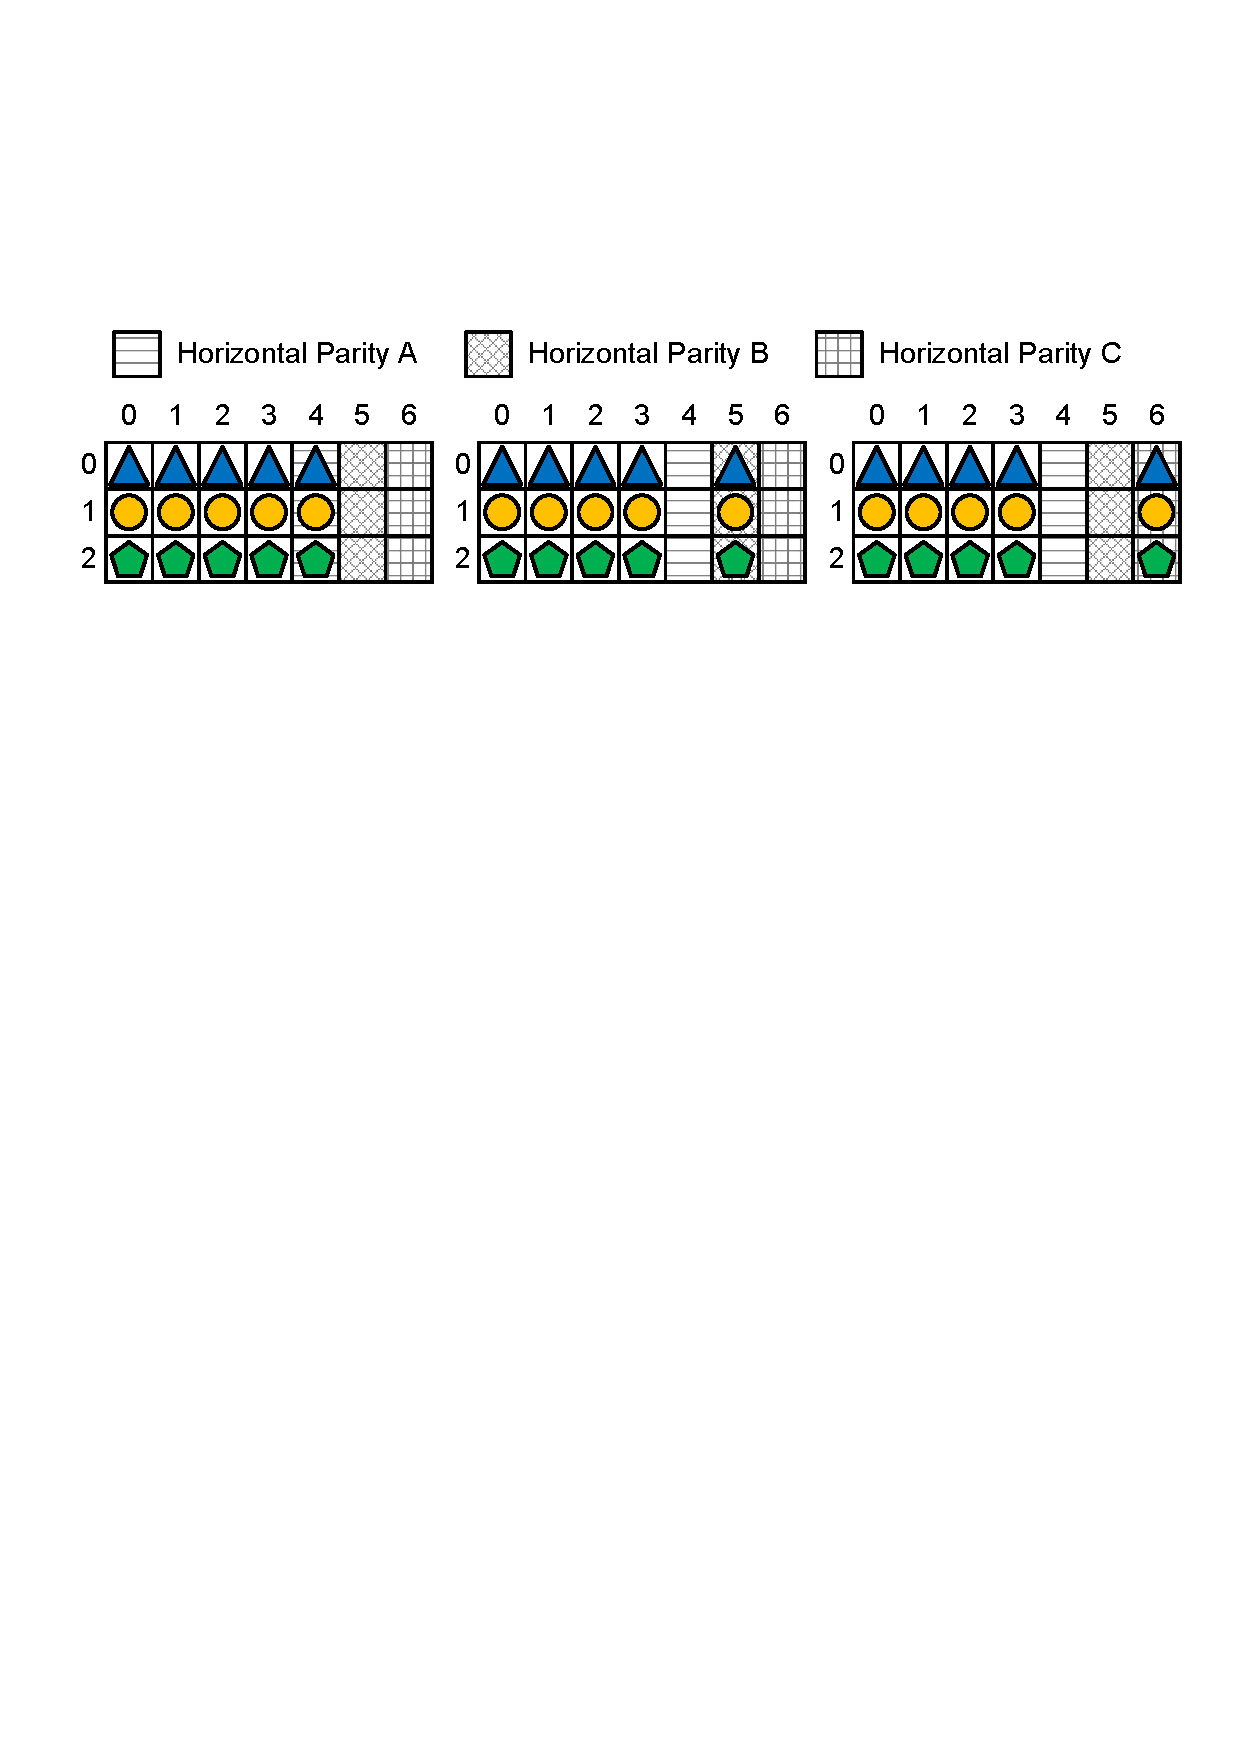
\includegraphics[width=0.26\linewidth]{photo/RS-1.pdf}\label{fig-RS-1}
    }
    \hspace{3px}
    \subfigure[\textbf{LRC Code:} Horizontal parity coding (e.g., the local parity $E_{0,5} = \sum_{i=2}^3 A_{0,i}E_{0,i}$ and the global parity $E_{0,7} = \sum_{i=0}^3 A_{0,i}E_{0,i}$)]{
        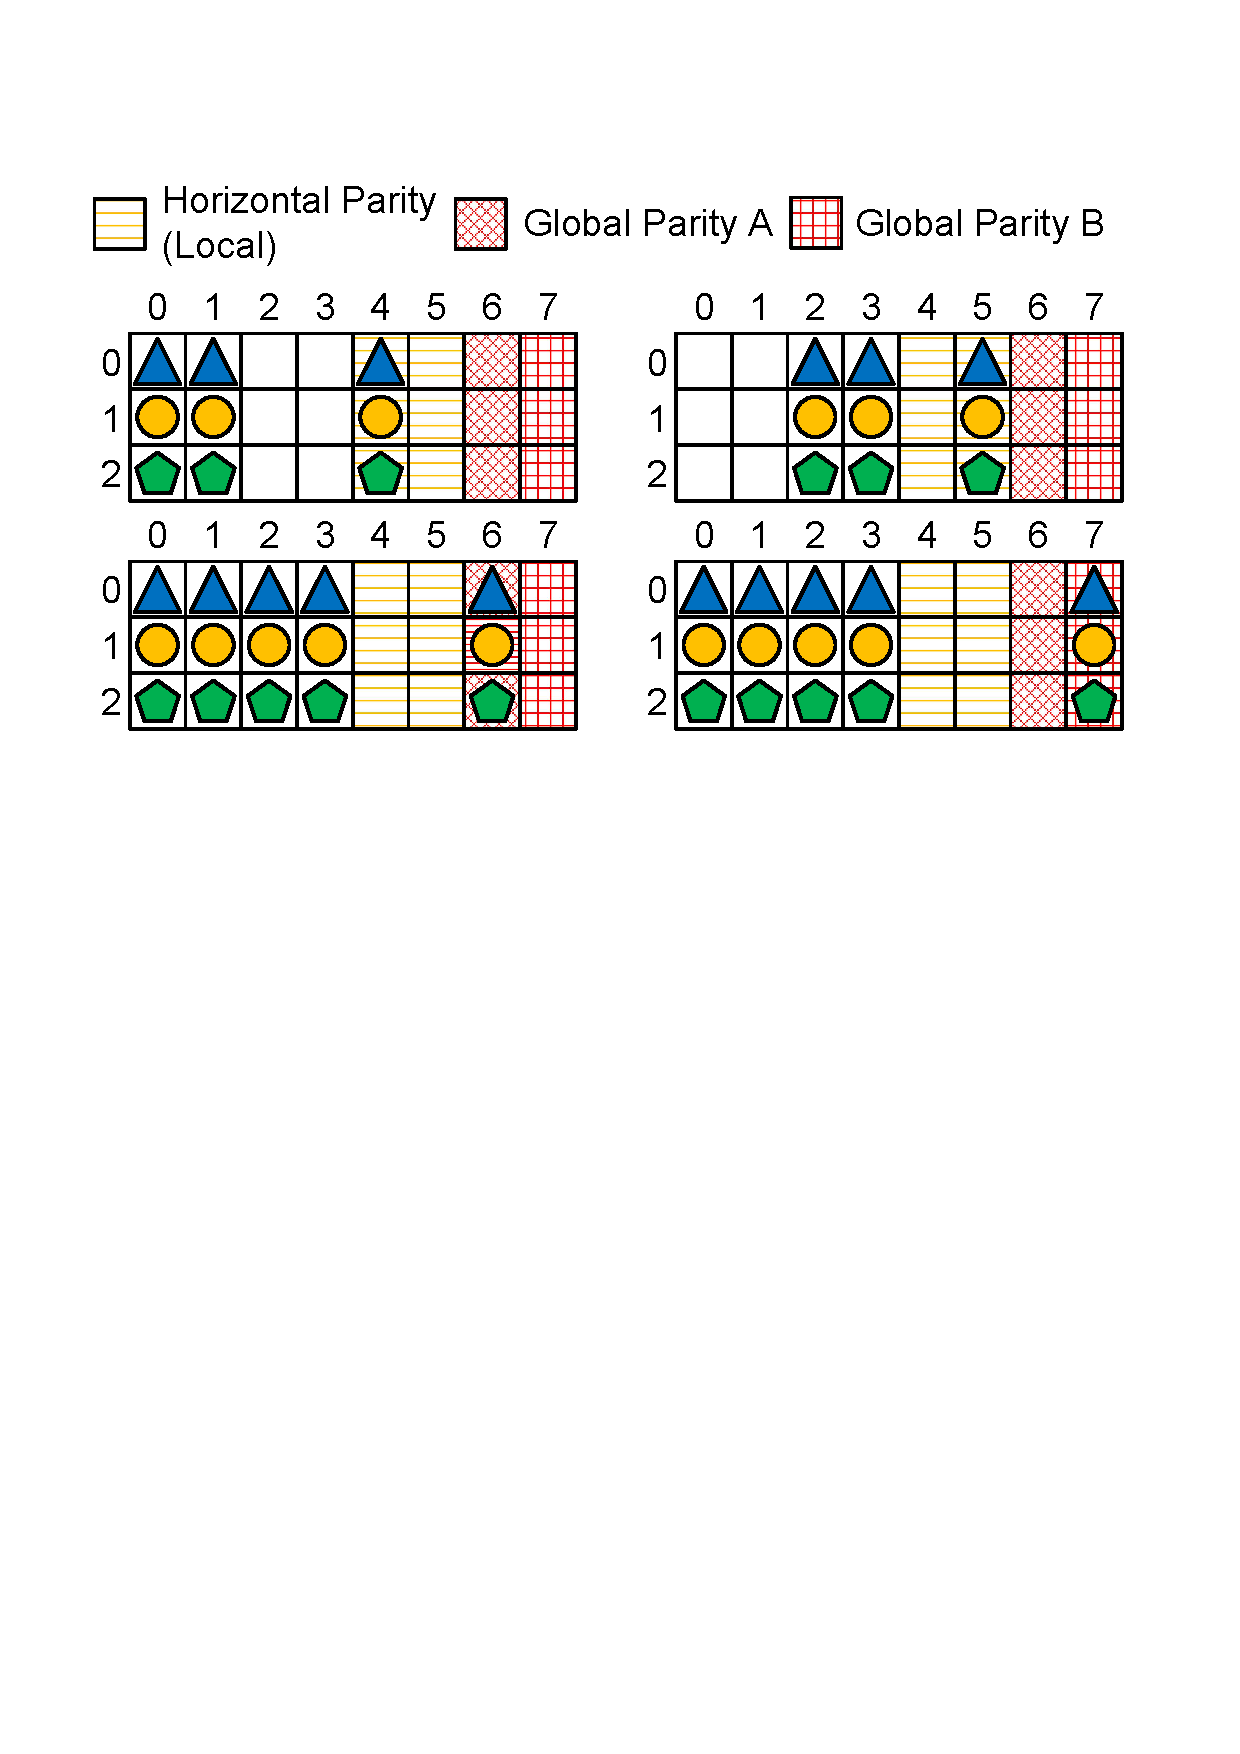
\includegraphics[width=0.67\linewidth]{photo/LRC-1.pdf}\label{fig-LRC-1}
    }
    \caption{Encoding of RS code and LRC}
\end{figure}

STAR code \cite{STAR} is an extension of the double-erasure-correcting EVENODD \cite{EVENODD} code, and a modification of the generalized triple-erasure-correcting EVENODD code. It employs a novice diagonal redundancy as shown in the left of Figure \ref{fig-star-tip}.

In the encoding process of STAR code, the generation of diagonal parity and anti-diagonal parity requires to calculate $S1$ and $S2$ first, which lead to a long parity chain.

\begin{figure}[!ht]
\centering
\subfigure[\textbf{STAR Code:} Horizontal parity coding (e.g., $E_{0,5} = E_{0,0} \oplus E_{0,1} \oplus E_{0,2} \oplus E_{0,3} \oplus E_{0,4}$).]{
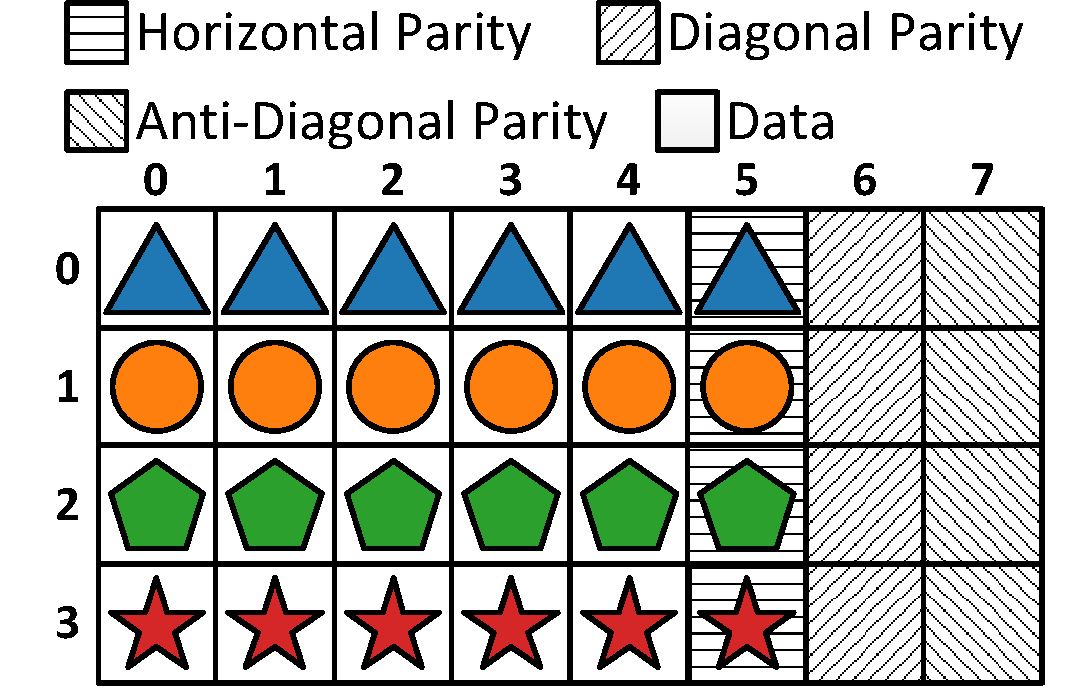
\includegraphics[width=0.42\linewidth]{photo/star-hori.pdf}\label{fig-star-1}
}
\hspace{5pt}
\subfigure[\textbf{STAR Code:} Diagonal parity coding (e.g., $S_1 = E_{3,1} \oplus E_{2,2} \oplus E_{1,3} \oplus E_{0,4}$ and $E_{0,6} = E_{0,0} \oplus E_{3,2} \oplus E_{2,3} \oplus E_{1,4} \oplus S_1$).]{
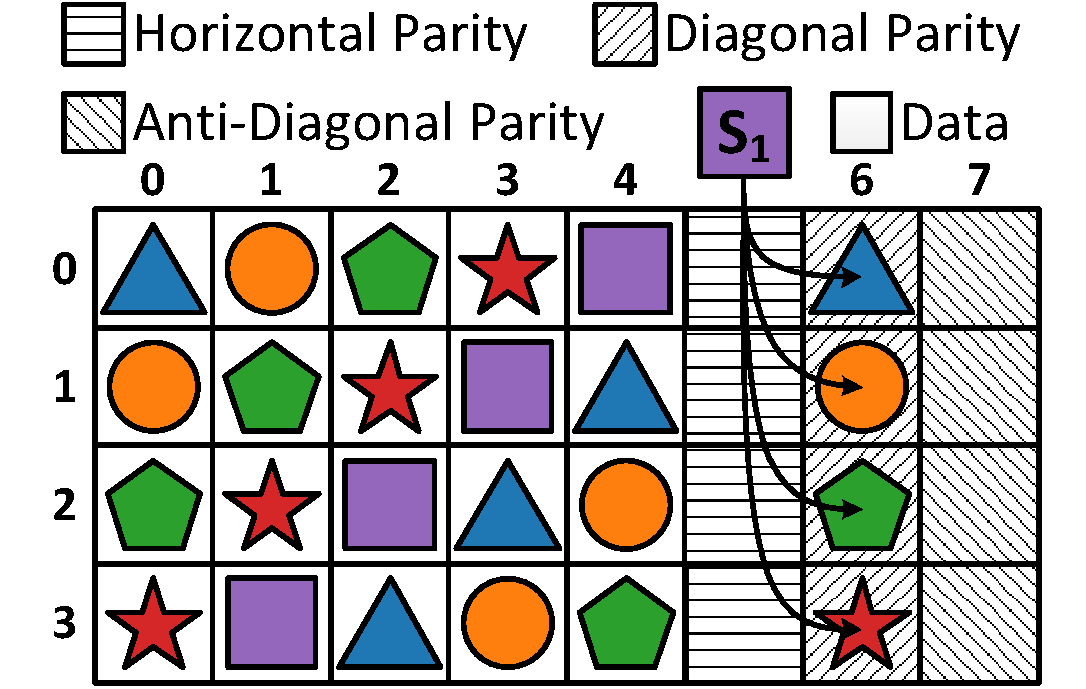
\includegraphics[width=0.42\linewidth]{photo/star-diag.pdf}\label{fig-star-2}
}

\subfigure[\textbf{STAR Code:} Anti-diagonal parity coding (e.g., $S_2 = E_{0,1} \oplus E_{1,2} \oplus E_{2,3} \oplus E_{3,4}$ and $E_{0,7} = E_{0,0} \oplus E_{1,1} \oplus E_{2,2} \oplus E_{3,3} \oplus S_2$).]{
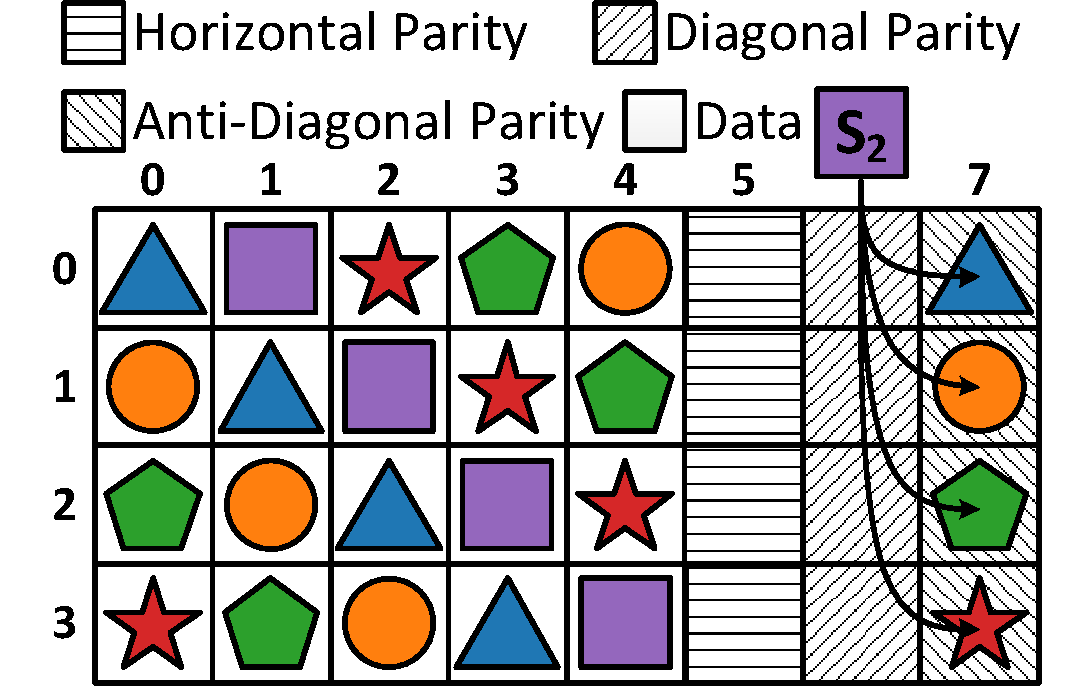
\includegraphics[width=0.42\linewidth]{photo/star-anti.pdf}\label{fig-star-3}
}
\hspace{5pt}
\subfigure[\textbf{TIP Code:} Horizontal parity coding (e.g., $E_{0,7} = E_{0,0} \oplus E_{0,2} \oplus E_{0,3} \oplus E_{0,4} \oplus E_{0,5}$).]{
\includegraphics[height=2.5cm]{photo/tip-hori.pdf}\label{fig-tip-1}
}

\subfigure[\textbf{TIP Code:} Diagonal parity coding (e.g., $E_{0,1} = E_{0,0} \oplus E_{5,2} \oplus E_{4,3} \oplus E_{2,5} \oplus E_{1,6}$ ).]{
\includegraphics[height=2.5cm]{photo/tip-diag.pdf}\label{fig-tip-2}
}
\hspace{5pt}
\subfigure[\textbf{TIP Code:} Anti-diagonal parity coding (e.g., $E_{0,6} = E_{0,0} \oplus E_{1,1} \oplus E_{2,2} \oplus E_{4,4} \oplus E_{5,5}$).]{
\includegraphics[height=2.5cm]{photo/tip-anti.pdf}\label{fig-tip-3}
}
\caption{Encoding of STAR (Figure \ref{fig-star-1}, \ref{fig-star-2} and \ref{fig-star-3}) and TIP (Figure \ref{fig-tip-1}, \ref{fig-tip-2} and \ref{fig-tip-3}) code ($p = 5$). Each column represents a node, each block represents an element, and parity chains are represented by elements with same shape.}
\label{fig-star-tip}
\end{figure}

TIP code is also an XOR-based 3DFTs erasure code.
Compared with STAR code, the encoding and data arrangement of TIP code eliminates the need to repeatedly calculate elements $S1$ and $S2$, so its cost of updating a single block is less than STAR code.

STAR requires the number of data nodes to be $p$, and TIP requires that to be $p-2$, where $p$ is a prime number.


\subsection{Approximate Storage \textcolor[rgb]{1.00,0.00,0.00}{Compression}}
%Storage techniques nowadays generally regard all information of the same importance, which causes significant costs in energy, disk drives and computing resources. But not all data need high-reliability storage for its backup. That is why the concept of approximate storage is introduced.
Approximate Storage is an innovative approach of trading off the limited resource budget with the costly reliability requirements, which recently receives more attentions since data centers are faced with storage pressure from the ever-increasing data.

Use cases for approximate storage range from transient memory to embedded settings and mass storage cloud servers. Mapping approximate data onto blocks that have exhausted their hardware error correction resources, for example, to extend memory endurance. On embedded settings, it enables the reduction of the cost of accesses and preserve battery life to loosen the capacity constraints. \cite{sampson2014approximate} Here, in data-center-scale video database, approximate storage can provide multiple levels of fault tolerance for data of different importance, avoiding redundant backup for the less-important data, thus saving a significant amount of space.


Approximate storage loosens the requirement of storage reliability by allowing quality loss of some specific data. Therefore, programmers can specify the importance of the data segments and assign them to different storage blocks. The critical data is still safe because they are stored and sufficiently backed up by expensive and highly reliable storage devices. Meanwhile, non-critical data is exposed to error, thus increasing storage density and saving cost.

%However, it is too naive to store data in approximate storage units indiscriminately. Related research \cite{guo2016high} shows that this can lead to unacceptable data pollution. To ensure data quality in this case, higher error correction costs are required resulting in an increase in overall storage costs. Therefore, it is very important to distinguish the importance of video data.

\begin{table}[ht]\footnotesize
\centering
\caption{
Comparison of storage overhead, reliability and performance among various storage methods for video files}\label{tab-AS-EC-AP}
\begin{tabular}{|c|c|p{1.2cm}<{\centering}|p{1.2cm}<{\centering}|p{1.2cm}<{\centering}|}
\hline
\multirow{2}{*}{EC} & RS & high & high & high \\ \cline{2-5}
 & RAID-6 & medium & medium & medium \\ \hline
\multicolumn{2}{|c|}{Approximate Storage} & low & low & low \\ \hline
\multirow{2}{*}{\begin{tabular}[c]{@{}c@{}}Approximate\\ Code\end{tabular}} & ID & low & high & low \\ \cline{2-5}
 & UD & low & medium & low \\ \hline
\multicolumn{2}{|c|}{Data Compression} & low & / & high \\ \hline
\end{tabular}
\end{table}





\subsection{Our Motivation}

%Based on Table \ref{tab-AS-EC-AP}, either the existing erasure codes or the approximate storage methods cannot meet the requirements of video applications in the cloud storage system due to the following reasons.
%First, the overhead of existing 3DFTs erasure codes is too high.
%Second, the 2DFTs erasure codes sacrifice part of reliability, and the reliability of approximate storage schemes are much lower since they cannot tolerate disk-level failures.
%Finally, existing erasure codes provide the same fault tolerance for all data without distinction, resulting in the same reliability for error-sensitive data and robust data.

From the summary of Table \ref{tab-AS-EC-AP}, we can find that existing solutions have high storage cost for video storage. Although approximate storage achieves low cost, the reliability cannot be satisfied in cloud environment. A feasible solution is combining the existing solutions together with tiered storage \cite{krish2014hats} \cite{wang2014balancing} \cite{zhang2010automated} \cite{udipi2012lot}, which motivates us to propose Approximate Code.

\begin{figure*}[ht!]
\centering
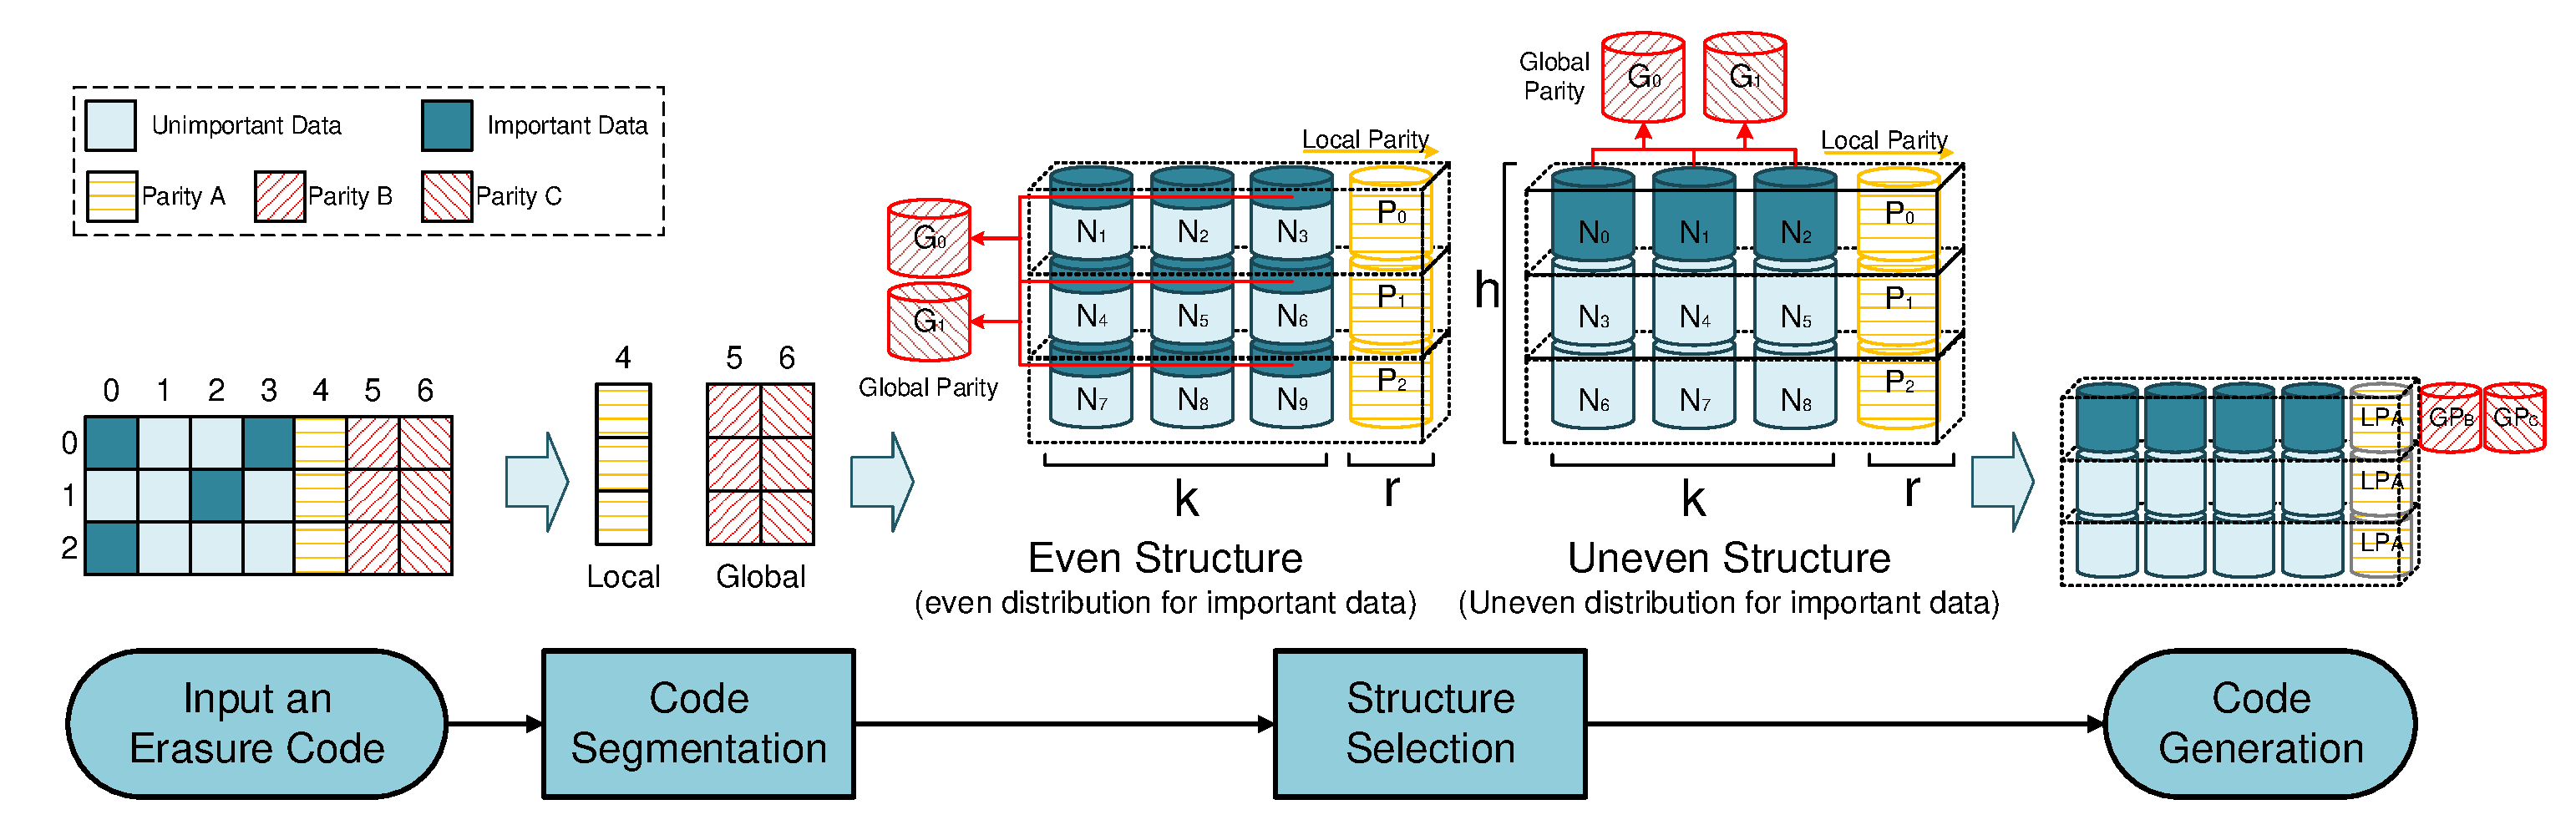
\includegraphics[width=0.9\linewidth]{photo/Framework-v3.pdf}
\caption{The framework of Approximate Code}
\label{fig-framework}
\end{figure*}

\section{Approximate Code}\label{ApCode}
In this section, we introduce the Approximate Code Framework and its properties through a few simple examples.

\subsection{Overview of Approximate Code Framework}
The Approximate Code framework contains four main steps, code input, code segementation, structure selection and code generation, as shown in Figure \ref{fig-framework}.

\subsubsection{Code Input}
Acquire an erasure coding input and get the corresponding parameters. Typically, for cloud storage systems, erasure codes used in 3DFTs are accepted by Approximate Code. Several parameters related to erasure codes need to be collected, such as the number of data nodes $k$ and the number of parity nodes $r$.

\subsubsection{Code Segmentation}
For an inputted erasure code, we assume that its fault tolerance is $x$. The Approximate Code first splits its parities into two parts: local and global parities. The former verifies all important and non-critical data, while the latter only verifies important data. Code segmentation are designed to ensure that local parities can tolerate any $r$ node failures, so the fault tolerance of non-critical data is $r$. For important data, the code segmentation ensures that the parity block of important data can be completely recombined into the original $x$DFTs erasure code scheme.

For example, several erasure codes in 3DFTs like STAR have three types of parities, horizontal, diagonal and anti-diagonal parities. In the code segmentation step, the horizontal parities are separated from other two parities.

\subsubsection{Structure Selection}
The Approximate Code framework then choose the structure for the input erasure code.
There are two main structures that distribute important and unimportant data in different ways.
As shown in Figure \ref{fig-framework}, in Even structure, important data occupies 1 block in each node, and in Uneven structure, it occupies 1 data stripe.
We specify that in Even structure, the ratio of important data to each node is $1/h$, thereby ensuring that the number of important data in both Even structure and Uneven structure just fills up $k$ nodes.

Since Even structure distributes important data across each node, it guarantees a more balanced load. Uneven structure concentrates important data into a stripe, and provides greater reliability for important data. A detailed analysis of this will be presented in Section \ref{ReconstructionFT}.

\subsubsection{Code Generation}\label{code-gen}
After code segmentation and structure selection, the Approximate Code Framework generates an approximate form of the input erasure code.
The construction of the Approximate Code is determined by 5 parameters $k$, $r$, $g$, $h$ and Structure.

We define the naming rules of the output Approximate Code as \textbf{APPR.CodeName} ($k,r,g,h$,Structure), where ``CodeName'' is the name of the input erasure code. Paremeter $Structure$ is Even or Uneven and it can be omitted when not focusing on the specific construction.

In a $n$-node stripe, $k$ of them are data nodes and $r=n-k$ nodes are for local parity, where each node can be divided into multiple blocks.
Approximate Code are designed for $h$ stripes, therefore it includes $k*h$ data nodes and $r*h$ local parity nodes.
Besides them, $g$ nodes are designed for global parity, which are calculated only by the important data blocks, so the total number of nodes $N$ in Approximate Code ($k,r,g,h$) is
$N= h*(k+r) + g$.

Approximate Code guarantees that the unimportant data can tolerate any $r$ node failures and the important data can tolerate any $r+g$ node failures.
Since the 3DFTs is a tipical configuration, we mainly discuss the situation of $r+g=3$, so $r$ is usually 1 or 2.

\subsection{\textcolor{red}{Approximate RS Code}}
For RS($k,p$), it can be seen that it provides $p$ independent horizontal parity nodes for $k$ data nodes. Therefore, the code segmentation for RS is arbitrary, that is, it supports any $r=p-g(0<g<p)$. RS also supports both two structures.

For the situation shown in Figure \ref{fig-framework}, we consider the input erasure code as RS($4,3$). It is divided into two local parities and one global parities with the Uneven structure and it generate Approximate RS Code ($4,2,1,3$,Uneven).
As a result, the unimportant data constitutes RS($4,2$), and the important data constitutes RS($4,3$).

\begin{figure}
    \centering
    \subfigure[XXX]{
        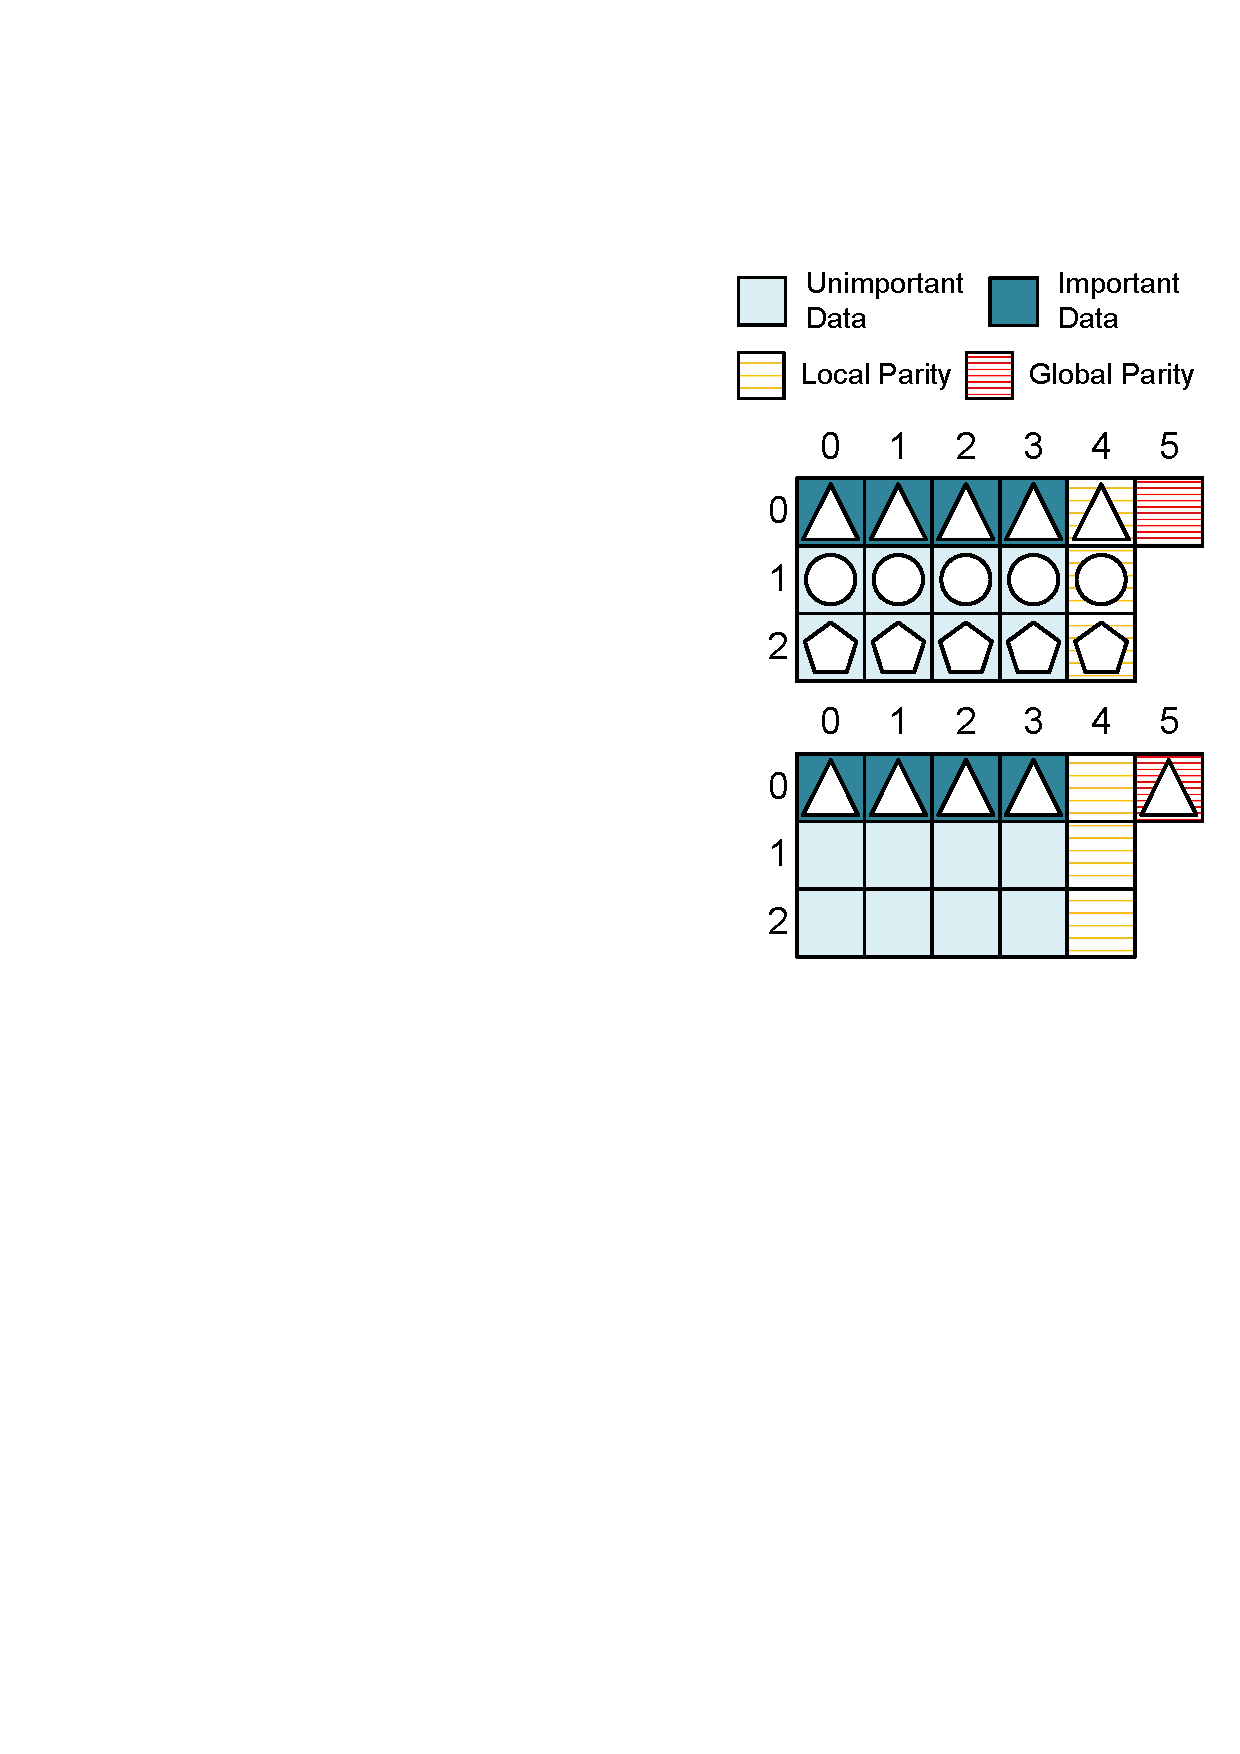
\includegraphics[width=0.26\linewidth]{photo/RS-2.pdf}\label{fig-RS-2}
    }
    \subfigure[XXX]{
        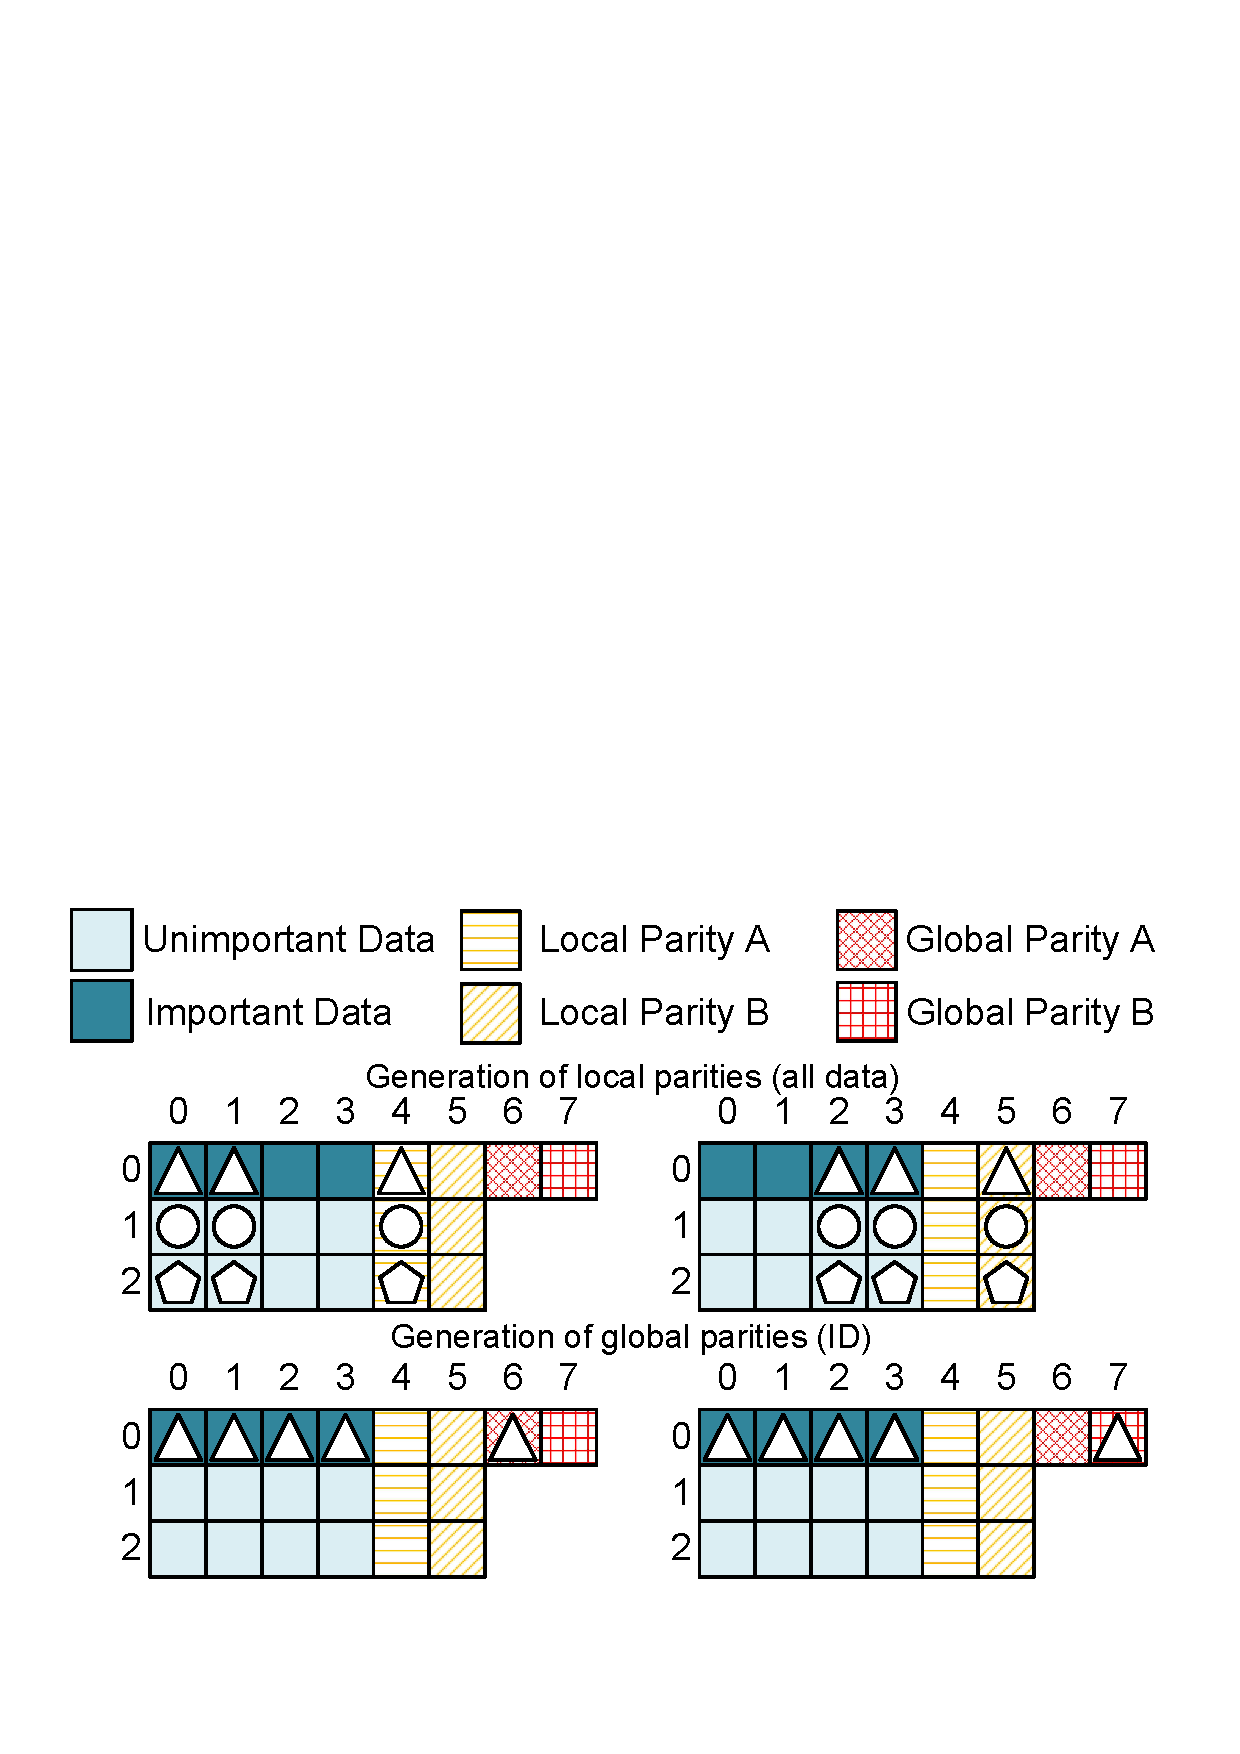
\includegraphics[width=0.68\linewidth]{photo/LRC-2.pdf}\label{fig-LRC-2}
    }
    \caption{XXXX}
\end{figure}

\subsection{Approximate XOR-based Codes}
Since we mainly provide 3DFTs for important data, we prefer to construct Approximate Code with several XOR-based codes to provide faster encoding and reconstruction speed than RS. This section introduce two tipical construction of Approximate XOR-based Code, Approximate STAR Code and Approximate TIP Code.

\begin{figure}[ht]
\centering
\subfigure[Structure selection of APPR.STAR Code]{
    \label{fig-ap-tip-str}
    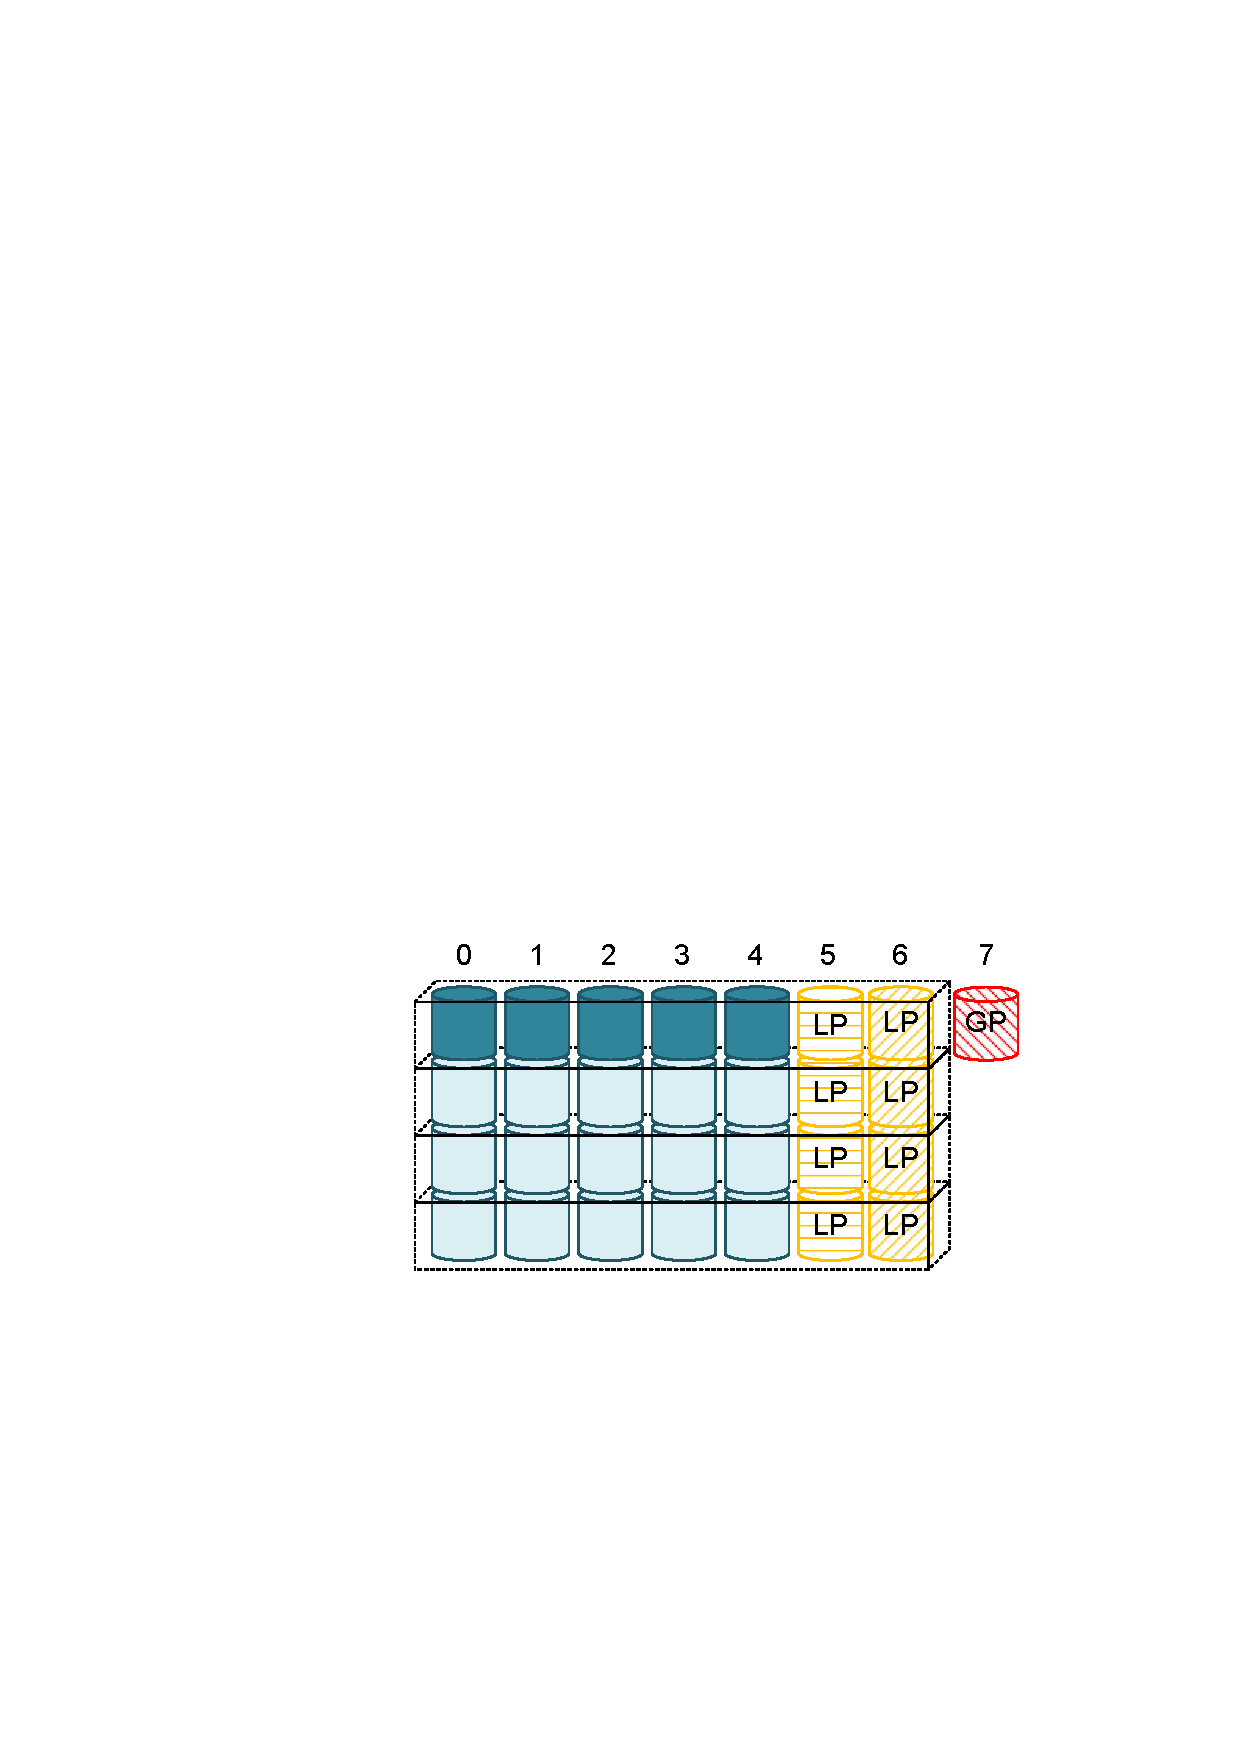
\includegraphics[width = 0.5\linewidth]{photo/APPR-STAR-STR.pdf}
}

\subfigure[Generation process]{
    \label{fig-ap-tip-GEN}
    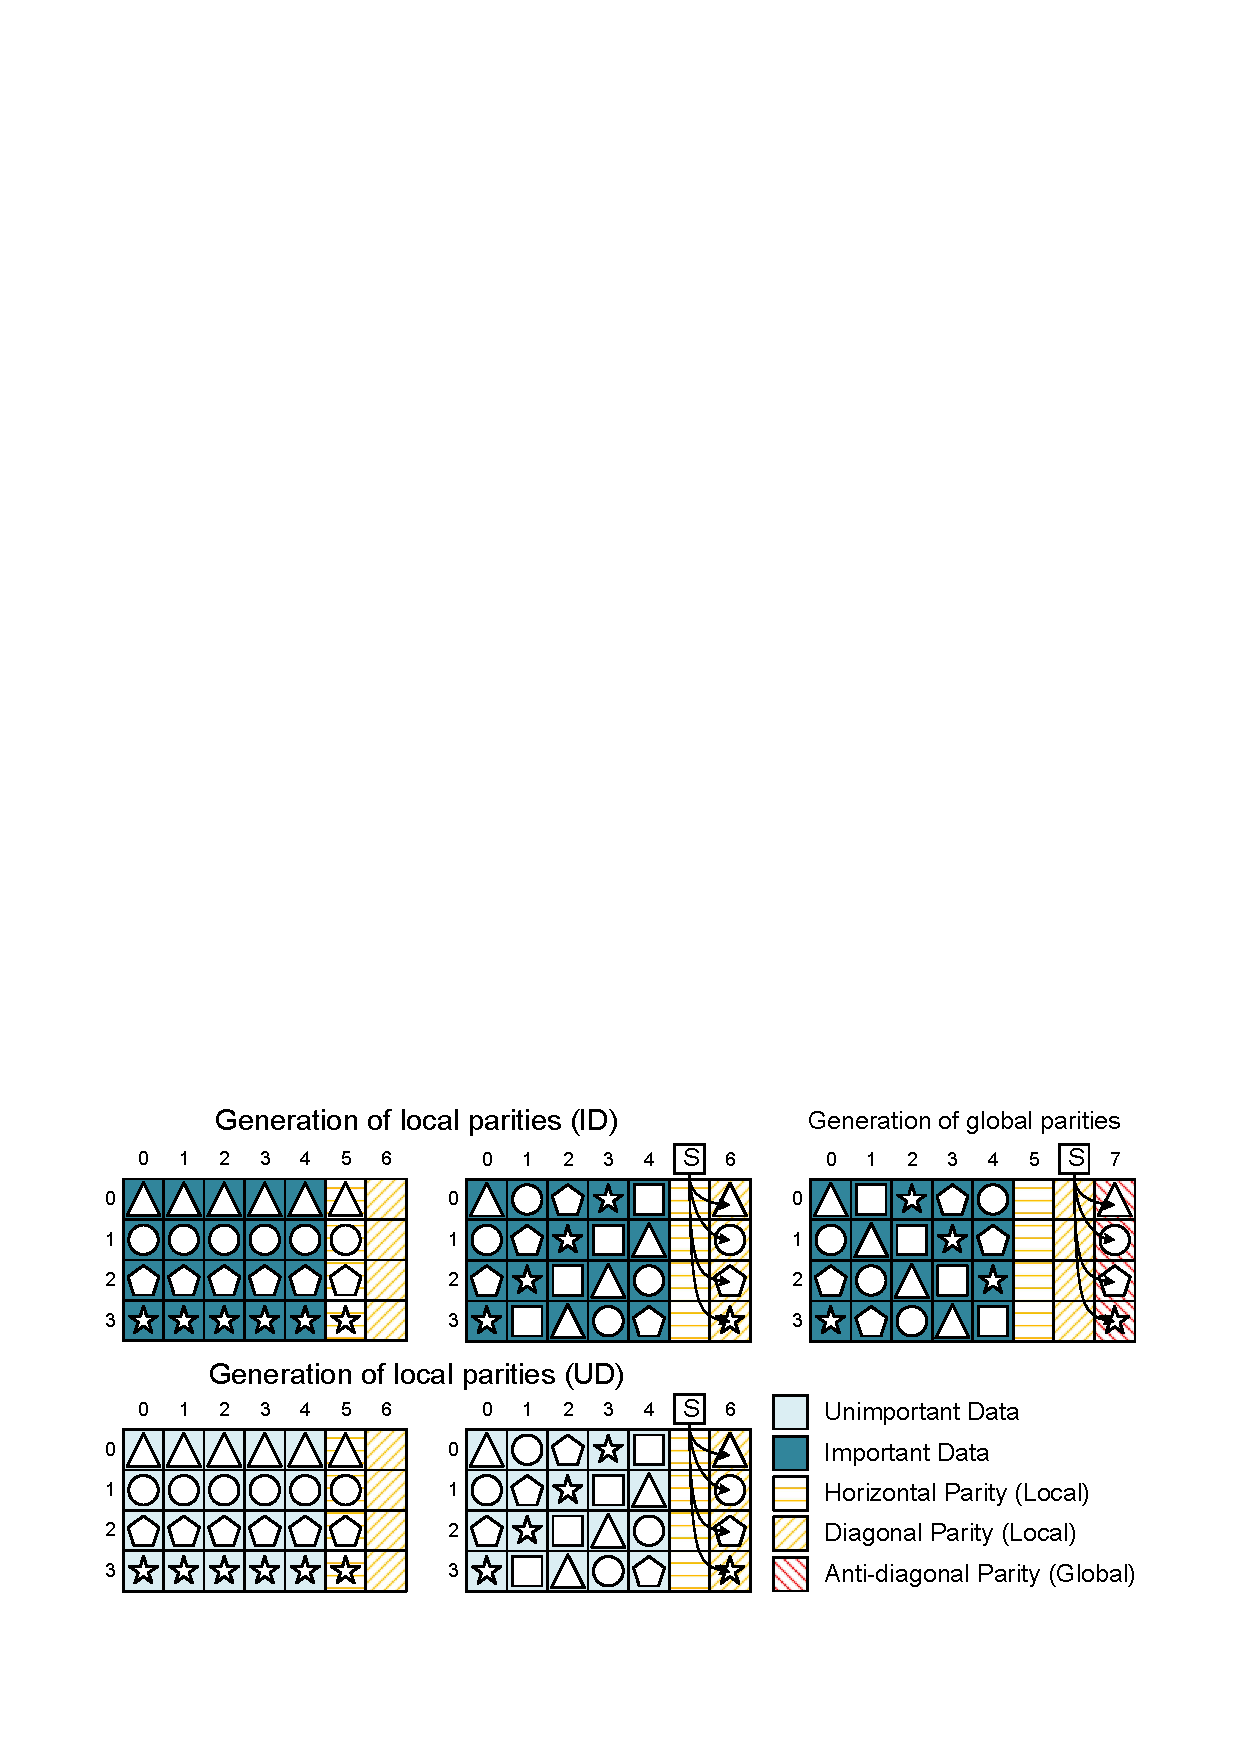
\includegraphics[width = \linewidth]{photo/APPR-STAR-GEN.pdf}
}
\caption{The construction and the encoding process of APPR.STAR ($5,2,1,4$,Uneven), which can be divided into STAR (encode important data) and EVENODD (encode unimportant data).}
\label{fig-ap-5214}
\end{figure}


\subsubsection{Approximate STAR Code}
Figure \ref{fig-ap-5214} shows the construction and the encoding process of APPR.STAR($5,2,1,4$,Uneven).
As introduced in \ref{existEC}, STAR Code \cite{STAR} has 3 parity chunks and it is a tipical 3DFTs XOR-based erasure code.
Since STAR is a direct extension of EVENODD\cite{EVENODD}, that is to say, STAR code that removes the anti-diagonal parity is the typical RAID-6 code EVENODD. As shown in Figure \ref{fig-ap-5214}, in this case, the horizontal and diagonal parity are used as local parities while the anti-diagonal parity is defined as global parity.
According to the construction requirements of STAR, each node is divided into 4 blocks.

Briefly, APPR.STAR($5,2,1,4$,Uneven) can be considered to be important data encoded by the full STAR, while the unimportant data is encoded by a portion of STAR, EVENODD. It is plain to see that important data can tolerate any 3 node failures while unimportant data can tolerate any 2 node failures.

\subsubsection{Approximate TIP Code}

\begin{figure}[ht]
\centering
\subfigure[Structure selection of APPR.TIP Code]{
    \label{fig-ap-tip-str}
    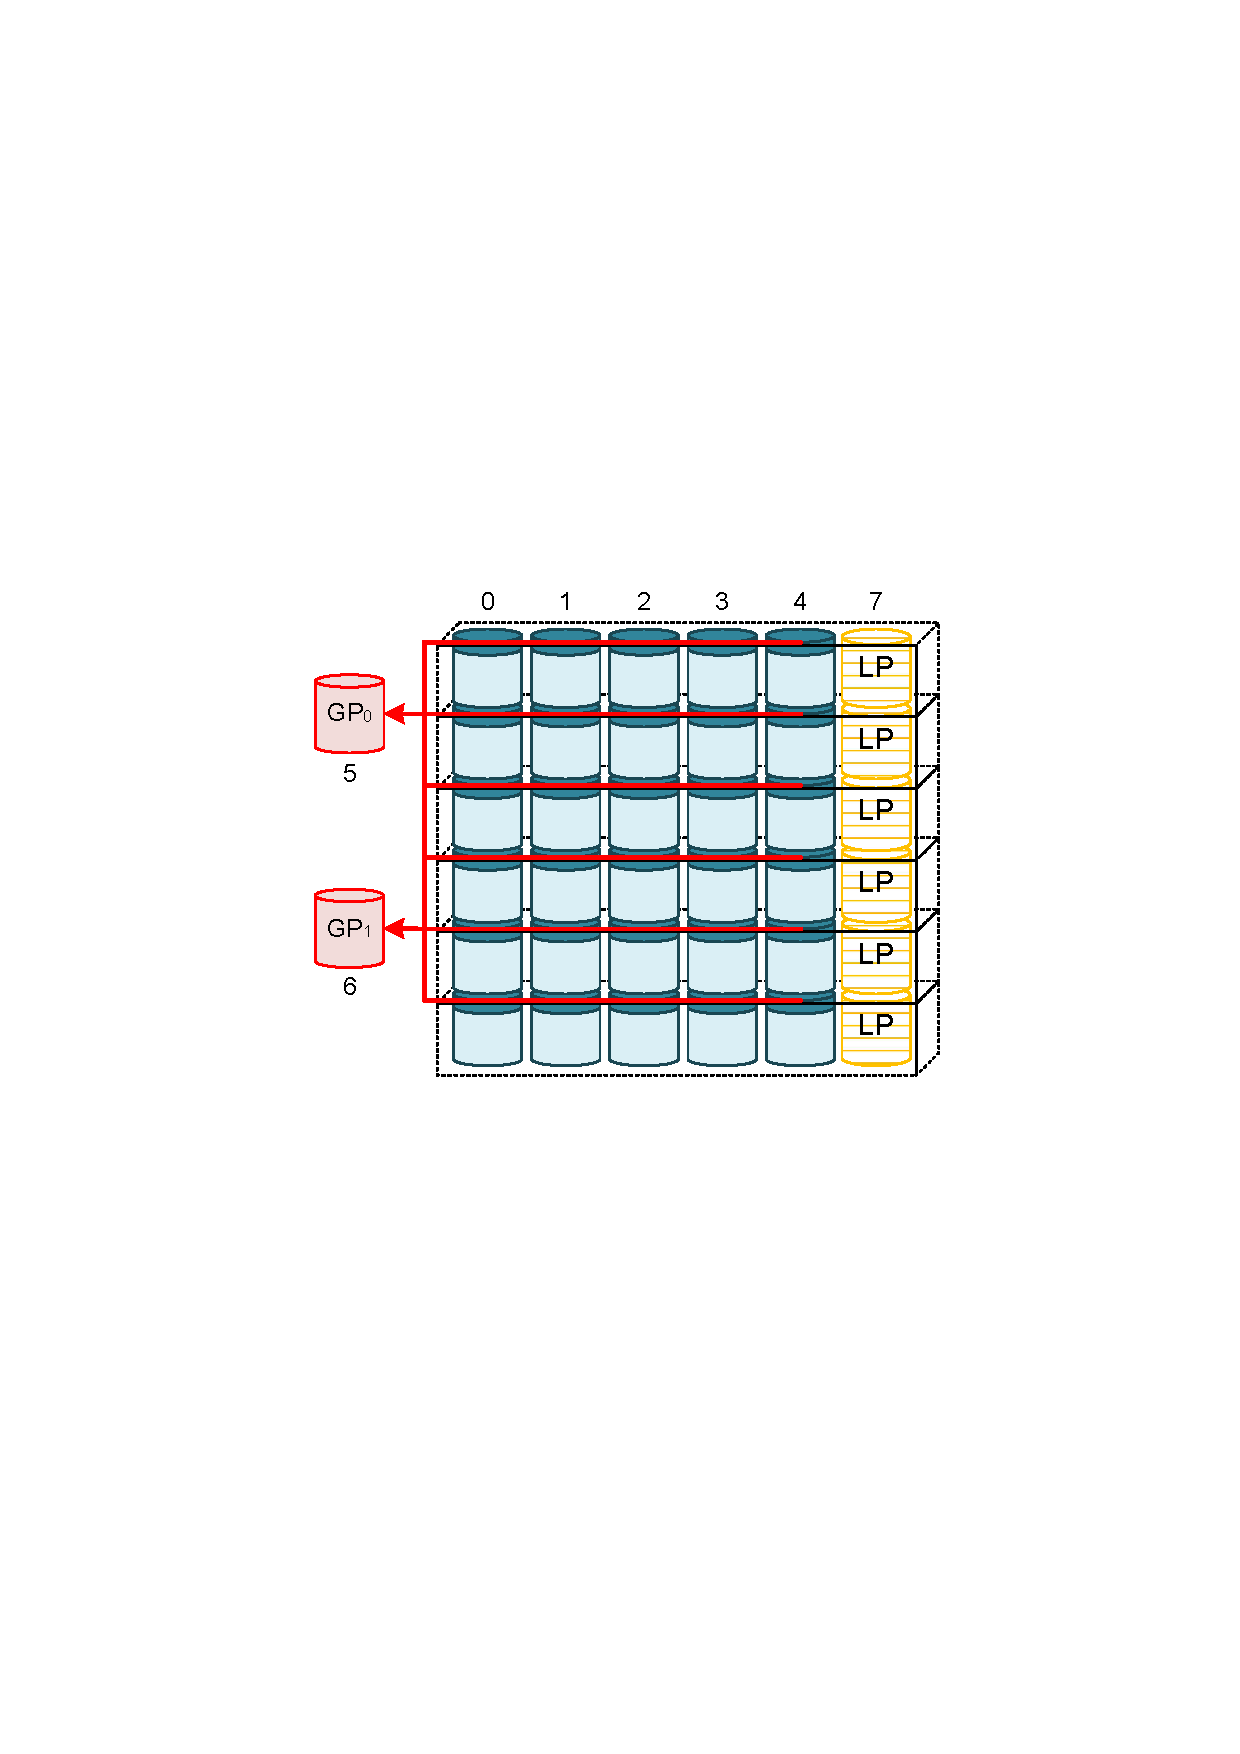
\includegraphics[width = 0.45\linewidth]{photo/APPR-TIP-STR.pdf}
}
\hspace{2pt}
\subfigure[Generation of local parities]{
    \label{fig-ap-tip-lP}
    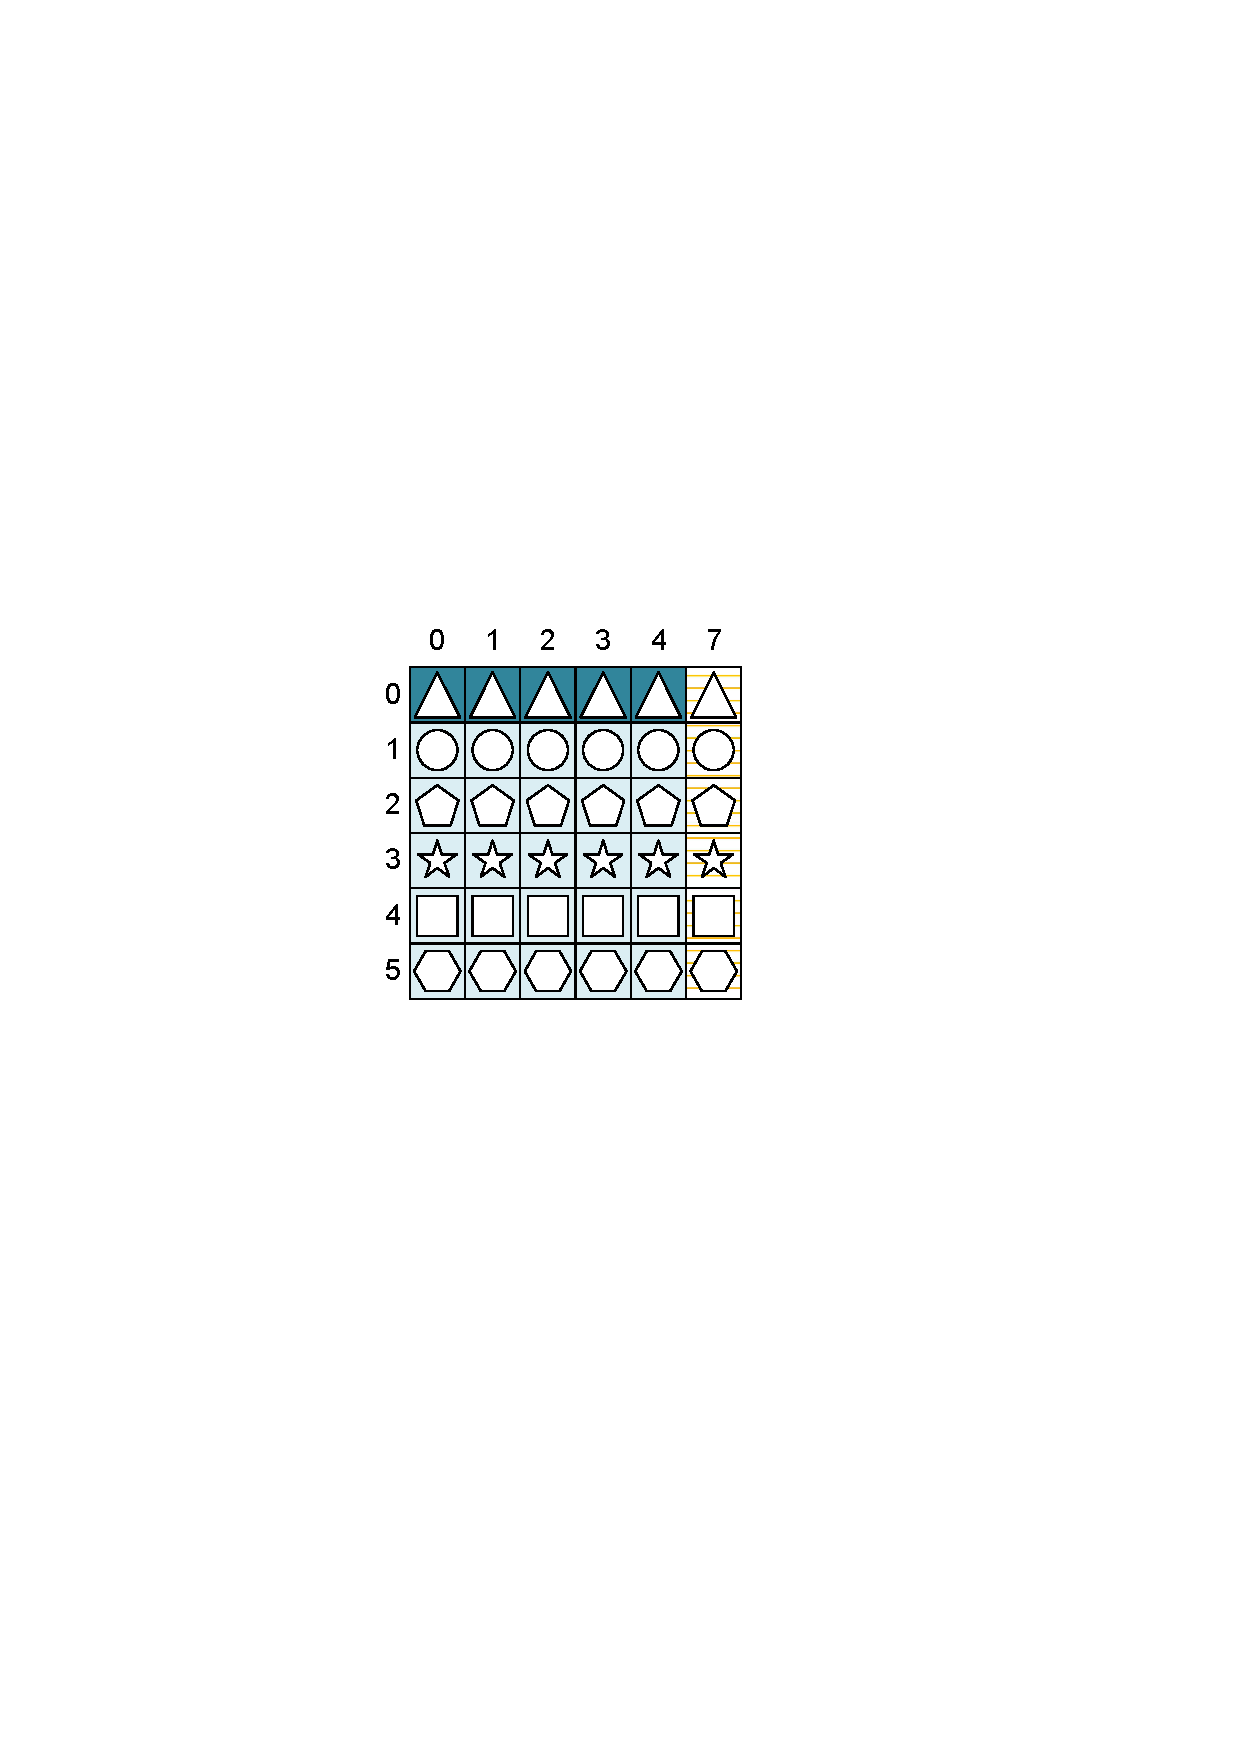
\includegraphics[width = 0.3\linewidth]{photo/APPR-TIP-LO.pdf}
}

\subfigure[Generation of global parities]{
    \label{fig-ap-tip-GP}
    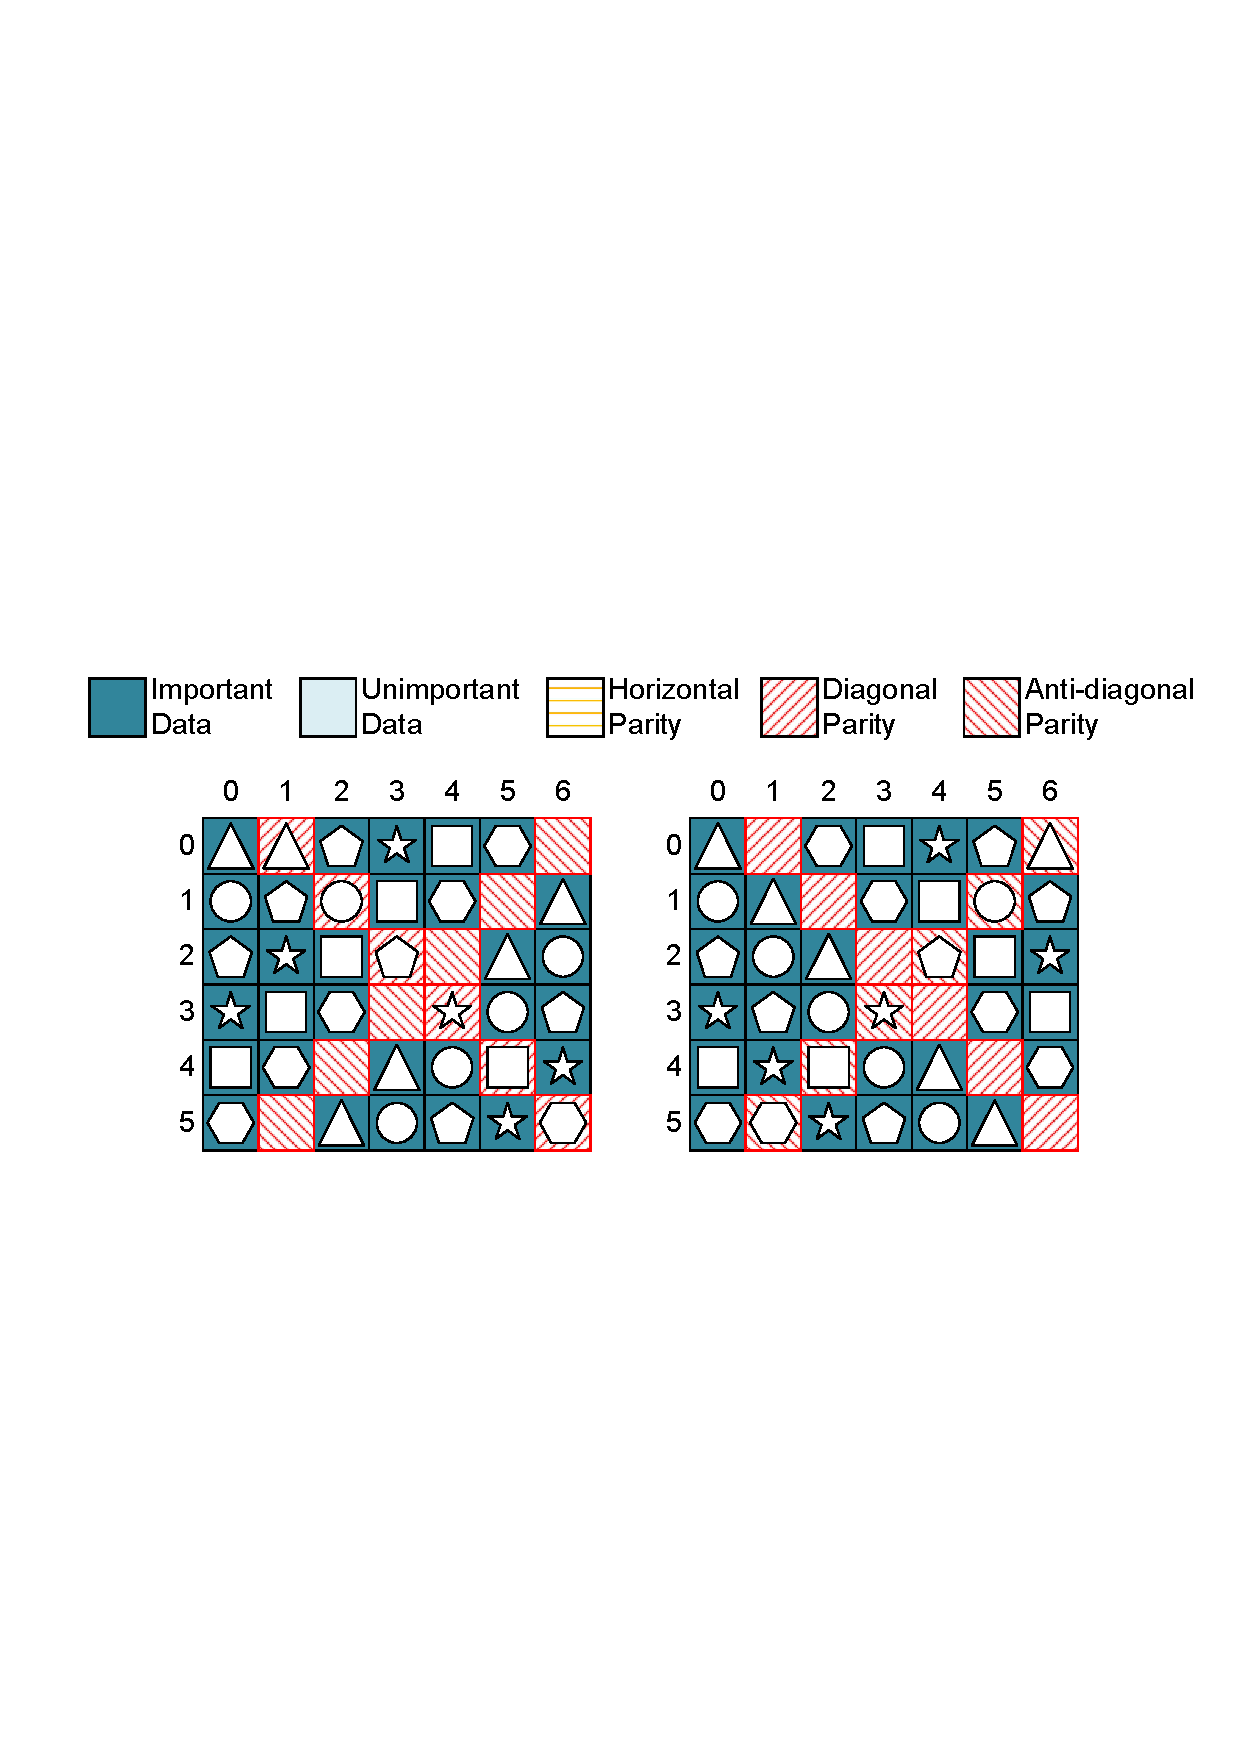
\includegraphics[width = 0.8\linewidth]{photo/APPR-TIP-GL-v2.pdf}
}
\caption{The construction and the encoding process of APPR.TIP ($5,1,2,6$,Even). The node 5 and 6 in TIP code is defined as the global parity nodes in this case.}
\label{fig-ap-TIP}
\end{figure}

We then introduce the generation of APPR.TIP($5,1,2,6$,Even).

In the code segmentation phase, we split TIP code into horizontal, diagonal and anti-diagonal parity. The important data is arranged in Even structure. However, since the parity block of the TIP is distributed over a series of nodes, the code generation process is different from that of the STAR.

We first generate local parity nodes by the horizontal parity for the important and unimportant data in each node. Then, we arrange the important data blocks as the type of Figure \ref{fig-tip-1}.
We use diagonal and anti-diagonal parity to encode the important data and define the last 2 node (Node 5 and 6) as the global parity nodes.

As shown in Figure \ref{fig-ap-TIP}, 30 data nodes form 6 stripes, where important data accounting for 1/6 of each node.
All data nodes generate 6 local parity nodes.
Important data blocks are rearranged to fit the parity form of TIP Code and generate two global parity nodes.

\subsection{Reconstruction Process and Fault Tolerance}\label{ReconstructionFT}
When $r$ or less nodes fail, all the data can be reconstructed by local parities.
When $r+g$ or less nodes fail, all the important data can be reconstructed by local and global parities.

However, in most cases, the loss of more nodes is also recoverable. We only consider two situations: $r+1$ and $r+g+1$.
The former exceeds the fault tolerance of unimportant data so we calculate the $P_{U}$, while the latter exceeds the fault tolerance of important data and we calculate the $P_{I}$.
As mentioned in Section\ref{code-gen}, $r+g$ is set to 3.

We exhaust all the conditions that may cause data loss and calculate the corresponding probability to calculate $P_{I}$ and $P_{U}$.
Approximate Codes based on different structures also have different fault tolerance and reconstruction cases, so we discuss Even structure and Uneven structure respectively.

\subsubsection{Lost $r+1$ nodes}
Under Even structure, the unimportant data nodes are recoverable as long as the node loss per stripe does not exceed $r$ and the global parity nodes do not need to be considered.
There are $\binom{N}{r+1}$ cases of loss of $r+1$ nodes and $h$ stripes in all. In each stripe, $\binom{k+r}{r+1}$ cases will result in unrecoverable of data.

Under Uneven structure, only $h-1$ stripes contain unimportant data, so $P_{U}$ is
\begin{align}
    P_{U-Even} &= 1 - \frac{h \times \binom{k+r}{r+1}}{\binom{N}{r+1}}\\
    P_{U-Uneven} &= 1 - \frac{(h-1) \times \binom{k+r}{r+1}}{\binom{N}{r+1}}
\end{align}

\subsubsection{Lost $4$ nodes}
The number of all 4-node lost cases is $\binom{N}{4}$.
We calculate the total number of cases in which all important data may be lost based on the different losses of the global parity nodes. The results are as follows:
\begin{align}
    P_{I-Even} = 1 - h*&\frac{\sum_{i=0}^{g} {\binom{k+r}{4-i}*\binom{g}{i}} }{\binom{N}{4}}  (g=1,2)\\
    P_{I-Uneven} &= 1 - \frac{\binom{k+3}{4}}{\binom{N}{4}}
\end{align}

According to the equations above, in Approximate RS ($3,1,2,3$, Even), $80.21\%$ 2-node failure cases are recoverable for unimportant data nodes, and $95.50\%$ 4-node failure is recoverable for important data nodes. In Approximate RS ($3,1,2,3$, Uneven), $P_U=86.81\%$ $P_{I}=98.50\%$.


\subsection{Properties of Approximate Code}\label{properties}

We analyze the nature of the Approximate Code from the following aspects, and the calculation method of the relevant indicators is given in Table \ref{tab-properties}.
\begin{itemize}
    \item Low Storage Overhead: Approximate Code reduces storage overhead by approximating and tiered storage strategies. This property is more pronounced for data with a smaller proportion of important data.
    \item Optimal Update Complexity: When one node is updated, Approximate RS Code only needs to write $r$ local parity nodes and only $g/h$ global parity nodes on average besides the write of data node.
    \item High reliability for important data. The Approximate Code guarantees 3DFTs for important data.
    \item Flexibility. The implementation of the Approximate Code can be based on RS, XOR or a mixture of the two.
\end{itemize}

\begin{table}[htb]
\centering
\caption{Comparison of storage overhead, fault tolerance and average single write performance between RS, STAR, TIP, Approximate RS, Approximate STAR and Approximate TIP}\label{tab-properties}
\begin{tabular}{|c|c|c|c|}
\hline
EC & \begin{tabular}[c]{@{}c@{}}Storage\\ Overhead\end{tabular} & \begin{tabular}[c]{@{}c@{}}Fault\\ Tolerance\end{tabular} & \begin{tabular}[c]{@{}c@{}}Ave Single Write\\ Overhead \end{tabular} \\ \hline
RS($k,r$) & $(k+r)/k$ & $r$ & $r+1$ \\ \hline
STAR($k,3$) & $(k+3)/k$ & $3$ & $6-\frac{4}{k}$ \\ \hline
TIP-code($k,3$) & $(k+3)/k$ & $3$ & 4 \\ \hline
\begin{tabular}[c]{@{}c@{}}APPR.RS\\ ($k,r,g,h$)\end{tabular} & \multirow{3}{*}{$\frac{(k+r)h+g}{kh}$} & $r+g$ & $1+r+\frac{g}{h}$ \\ \cline{1-1} \cline{3-4}
\begin{tabular}[c]{@{}c@{}}APPR.STAR\\ ($k,2,1,h$)\end{tabular} &  & 3 & $2\frac{k-h-1}{kh}+4$ \\ \cline{1-1} \cline{3-4}
\begin{tabular}[c]{@{}c@{}}APPR.TIP\\ ($k,1,2,h$)\end{tabular} &  & 3 & $2+\frac{2}{h}$ \\ \hline
\end{tabular}
\end{table}

\subsection{Implementation}\label{Implementation}
\begin{figure}[htb]
\centering
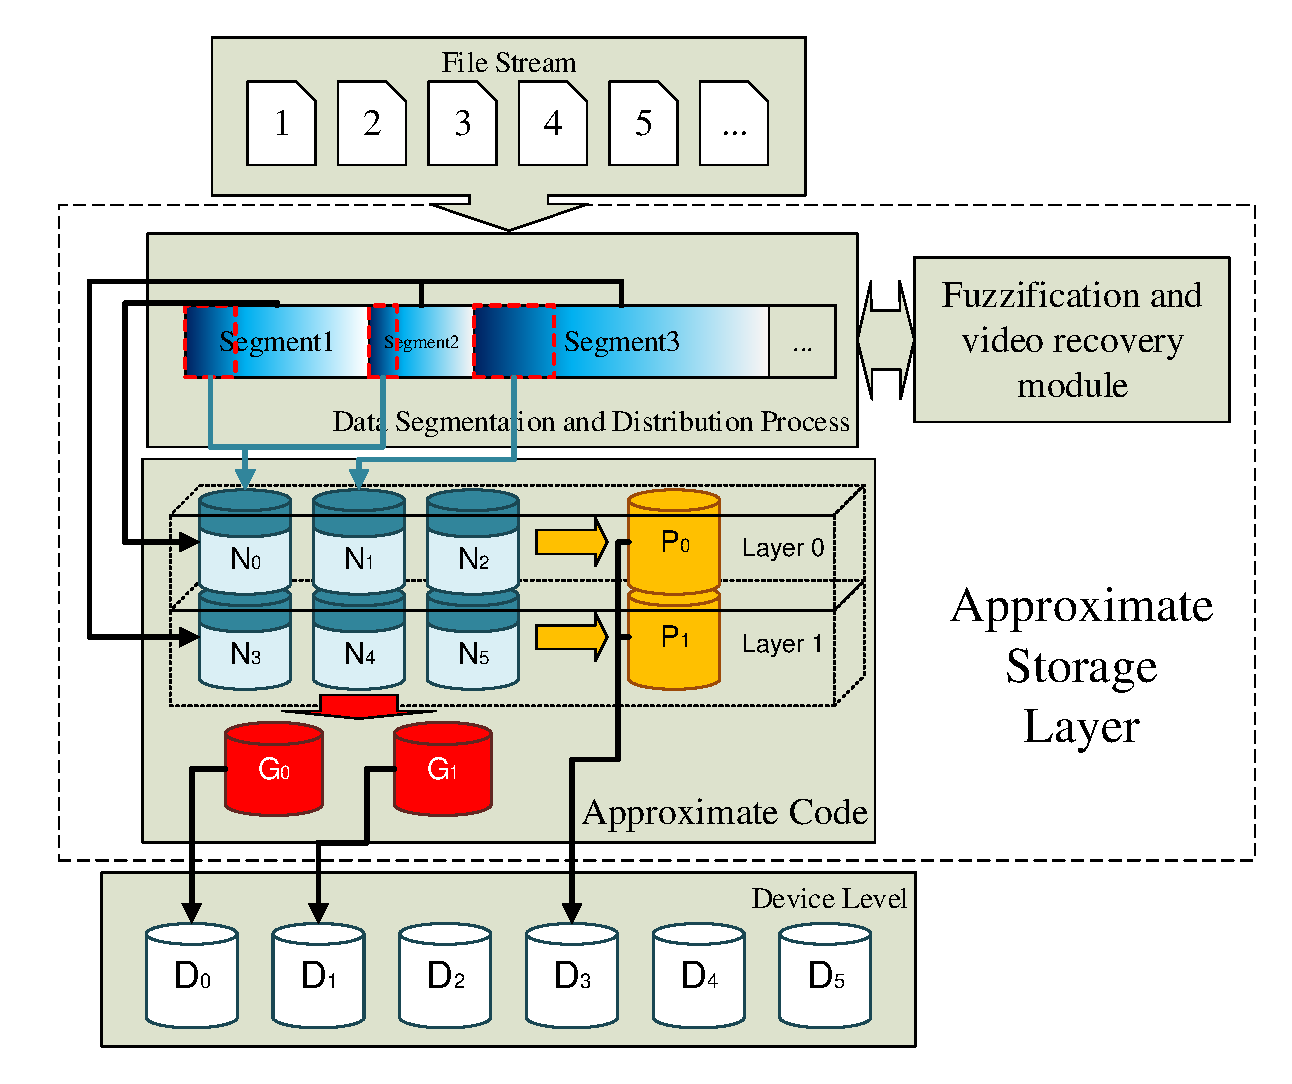
\includegraphics[height = 5.5cm]{photo/implementation-V2.pdf}
\caption{Overview of Approximate Storage Layer}
\label{fig-implementation}
\end{figure}

Compared with the traditional scheme that does not consider the meaning of the upper layer data, the Approximate Code pays attention to the difference of the importance of the data, so an intermediate layer between the upper layer application and the underlying distributed storage system is necessary. We call it the approximate storage layer, which include 3 parts: data identification and allocation, encoding and decoding process of Approximate Code and the video fuzzification and recovery.

\subsubsection{Data Segmentation and Distribution module}
The data segmentation module splits the video file stream into multiple data segments and automatically discriminates the important data. A natural approach is to follow the GOP segmentation. According to the \ref{video storage}, the GOP of the encoded video starts with an I frame, and all the data in that GOP depends on it for decoding, so we define it as important data and divide the GOP into I frames (important part) and other data. (unimportant part).
%The data distribution module distributes important data and unimportant data in different blocks and records the location. This location information is also defined as important data.
This module is also responsible for analyzing the proportion of important data and unimportant data in the data stream to select the most appropriate coding parameter configuration to ensure fault tolerance and high storage efficiency of important data.

\subsubsection{Approximate Code module}
The Approximate Code module is responsible for encoding and decoding important and unimportant data and completely recovering the data within fault tolerance. For data that cannot be recovered, the Approximate Code module transmits it to the video recovery module for approximate recover videos.
%Approximate Code module is also responsible for allocating blocks of data to ensure that blocks of each stripe are distributed to different nodes, while ensuring that global check blocks and data blocks are not on one node.

\subsubsection{Data Fuzzification and Video Recovery}
In the approximate recovery mode, the remaining data and important data are transferred to this module. Using a series of methods described in Section \ref{video storage}, frames that suffer from frame loss will be recovered using the interpolation algorithm; the corrupted frames will be processed into fuzzy images and approximately recovered by superpixel techniques.


\section{Evaluation}\label{evaluation}
In this section, we conduct a series of experiments to demonstrate the efficiency of Approximate Code.
\subsection{Evaluation Methodology}
The experiment is divided into two parts: the first part evaluates the performance of the Approximate Code code, and the second part evaluates the impact of the loss of the unimportant data on the video files.

To compared with Approximate Code, We choose several 3DFTs erasure codes, including RS code, LRC, STAR and TIP code.
Experiments as well as mathematical analysis are used to demonstrate the performance of Approximate Code.

To prove that the lost of unimportant data is acceptable, we use the latest interpolation algorithm to simulate the approximate recovery and fuzzification process in a data corruption scenario.

\subsubsection{Metrics and Methods for Mathematical Analysis: }
We use the \textbf{Storage Efficiency}, \textbf{Fault Tolerance} and \textbf{Single Write(update) Cost} defined in Table \ref{tab-properties} as measure.
We first analyze the impact of the settings of the three parameters on these metrics, then we compare these matrics with several EC methods.

\subsubsection{Metrics and Methods for Experiments: }
We use \textbf{Encoding Time} and \textbf{Recovery Time} as the metrics in our experiments. Encoding Time is the time for generating all parity nodes and Recovery Time is the time for recovering the lost nodes.

In our experiments of recovery time, we compare Approximate Code with several other codes with the same data nodes $k$.
Note that the Approximate Code can only recover important data in some cases, and we don't consider the recovery of non-critical data, so the Approximate Code may recover less data than other codes.

The environment of our experiments are shown in Table \ref{tab-platform}. We set a Hadoop system with one NameNode and $h$ DataNodes. Each DataNodes storage the data of one layer of Approximate Code and the global parities are distributed at each DataNodes. We set $h=4,6$ and node size equal $1GB$ here as two default configurations.

Our experiment can mainly be divided into four cases. First, we evaluate the encoding time for several erasure codes. We then evaluate the recovery time of the scenarios where single, double and triple nodes are corrupted.

\subsubsection{\textcolor{red}{Metrics and Methods for Frame Recovery: }}
we performed the experiment of video frame recovery with the frame interpolation technique. The dataset we used is a collection of 60fps videos from \textbf{YouTube-8m} \cite{youtube8m}. We simulated a 1\% data loss\footnote{In a distributed system, a single video can be stored in dozens or even hundreds of nodes. We assume that its important data is recovered, while the loss of unimportant data accounts for 1\% of the total video size.} on the less important video frames and successfully recovered the lost ones, although the recovered frames have some discrepancies with the original data. The average quality of the recovered pictures is commonly above 35dB in terms of Peak Signal to Noise Ratio PSNR .

\begin{table}[!ht]
\begin{tabular}{|l|l|}
\hline
Description & DELL R730 Server \\ \hline
CPU & Intel Xeon 3.0GHz \\ \hline
NIC 1Gbps & 1Gbps \\ \hline
Memory & 32GB \\ \hline
Disk & 8TB HDD \\ \hline
OS & Linux 3.19 \\ \hline
Platform & Hadoop HDFS 3.0.3 \\ \hline
\end{tabular}
\caption{Details of Our Evaluation Platform}\label{tab-platform}
\end{table}

\subsection{Numerical Results of Mathematical Analysis}
\subsubsection{Storage Overhead}
We compare the storage overhead between RS ($k,3$), APPR.RS ($k,1,2,h$) and APPR.RS ($k,2,1,h$), where $h = 4$ or $6$.
As shown in Figure \ref{fig-Storage}, the results shows that APPR.RS Code has much lower storage overhead than RS Code. The ratio of optimization is up to 21.4\% when $h=4, k=4$ and $23.8\%$ when $h=6, k=4$. For more tipical configuration that $k=6$, APPR.RS ($6,1,2,4$) recude the number of parity nodes from $3$ to $1.33$.

\subsubsection{Fault Tolerance}
All the erasure codes we evaluate in this Section are 3DFTs.

\subsubsection{Single Write Performance}
We compare the single write performance between RS, STAR, APPR.RS and APPR.STAR, where $h = 4 or 6$. As shown in Figure \ref{fig-Sig-Write}, the results shows that APPR.RS Code has lower single write performance than RS Code and STAR Code. The ratio of optimization is up to $41.3\%$ when $h=6$ and $25\%$ when $h=4$. As $k$ increases, the performance of APPR.STAR is close to RS and always better than STAR.

\begin{figure}[ht]
\subfigure[h=4]{
    \label{fig-storage4}
    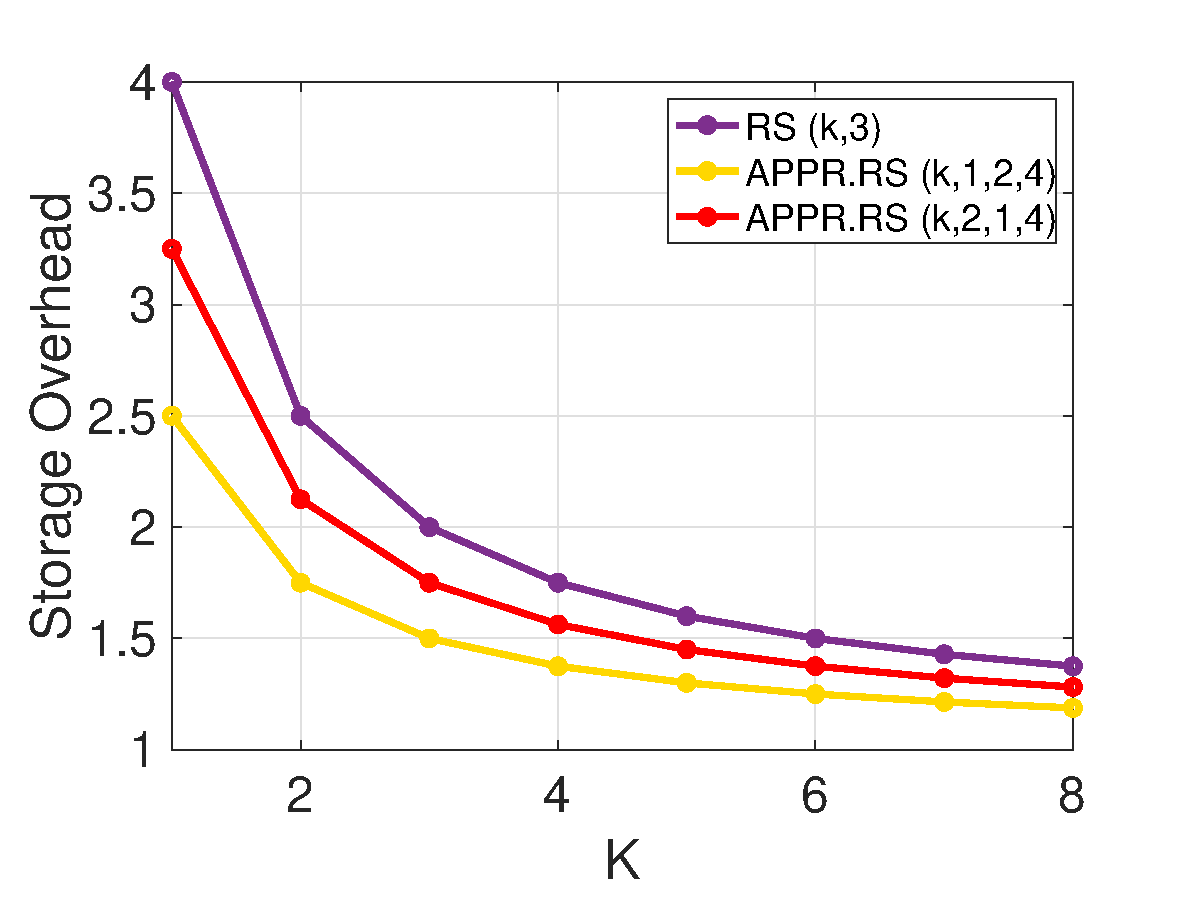
\includegraphics[width = 0.44\linewidth]{photo/experiment/Storage-4.eps}
}
\subfigure[h=6]{
    \label{fig-storage6}
    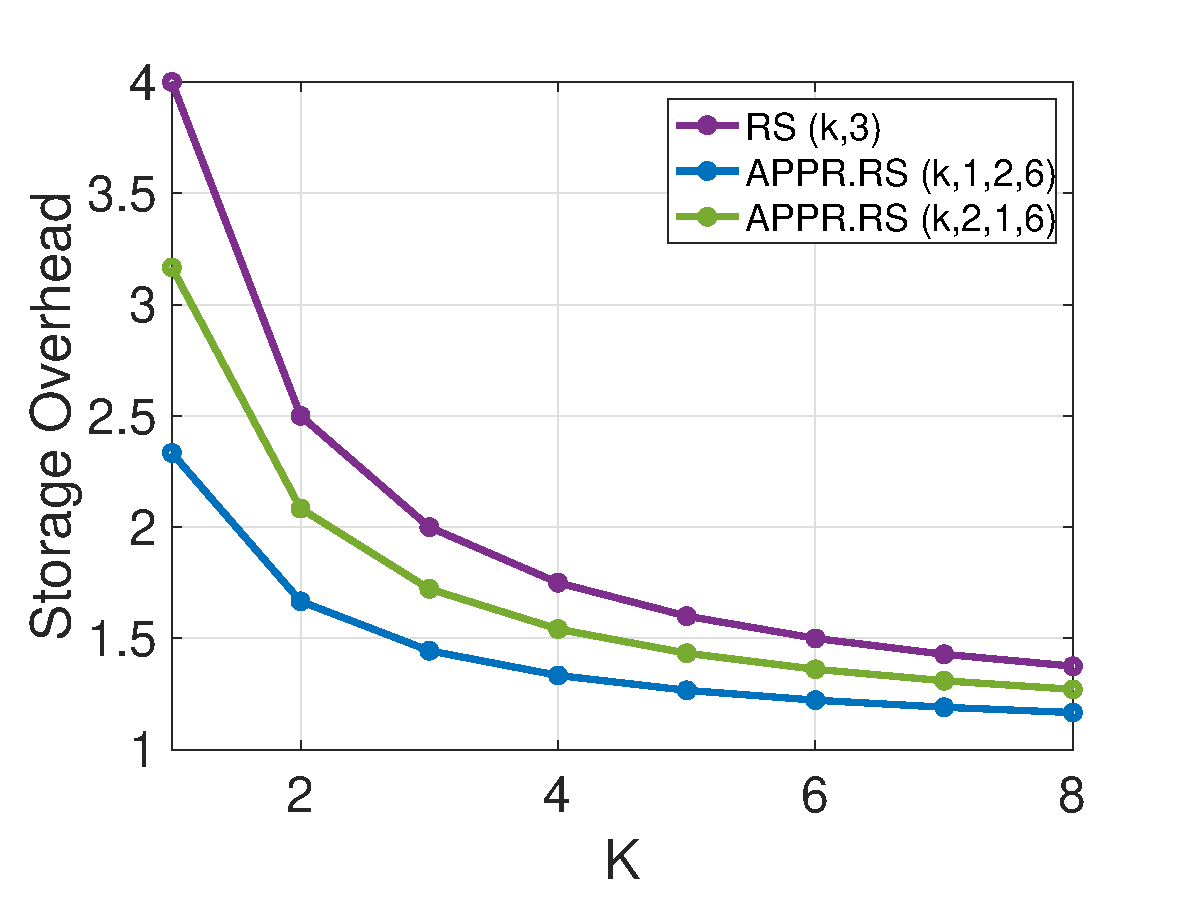
\includegraphics[width = 0.44\linewidth]{photo/experiment/Storage-6.eps}
}
\caption{Storage Overhead}\label{fig-Storage}
\end{figure}

\begin{figure}[ht]
\subfigure[h=4]{
    \label{fig-Sig-Write4}
    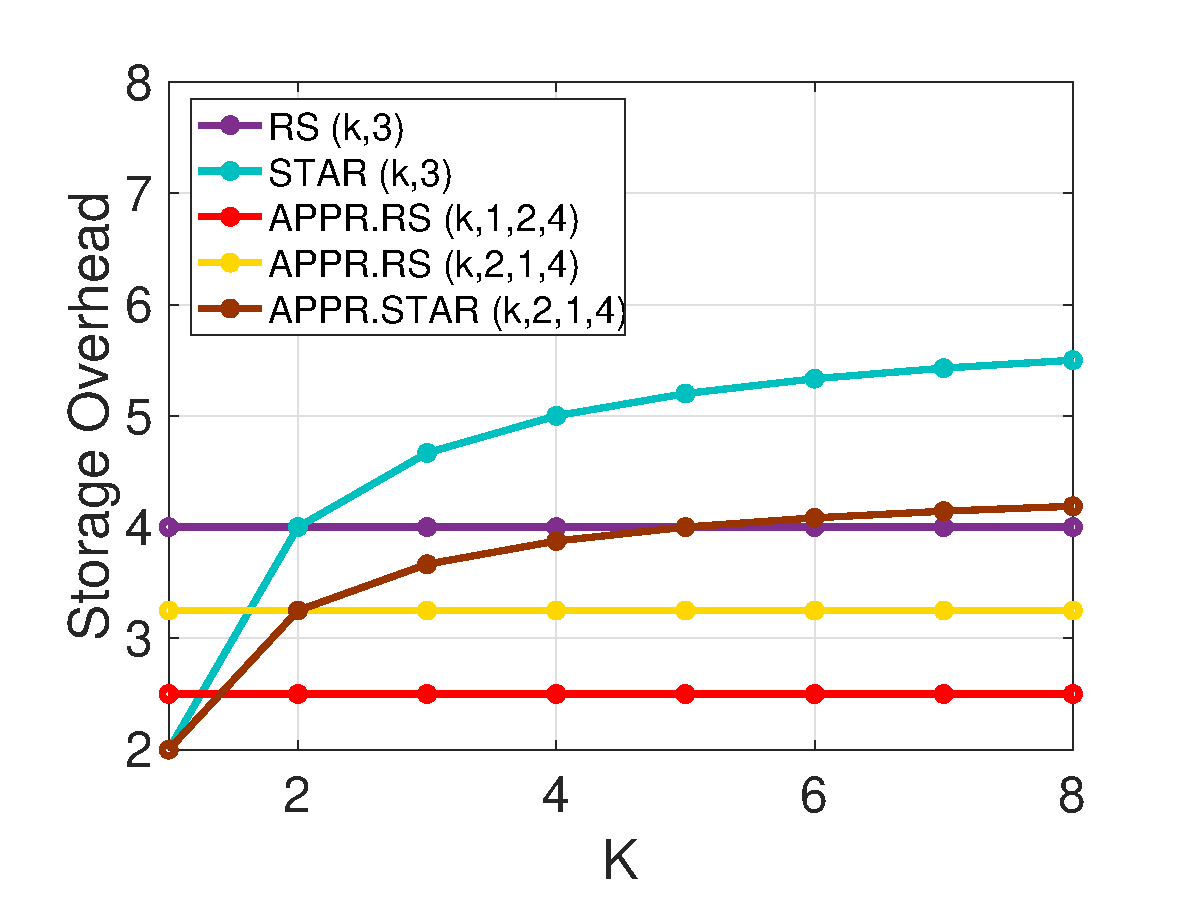
\includegraphics[width = 0.44\linewidth]{photo/experiment/Single-4.eps}
}
\subfigure[h=6]{
    \label{fig-Sig-Write6}
    \includegraphics[width = 0.44\linewidth]{photo/experiment/Single-6.eps}
}
\caption{Single Write Performance}\label{fig-Sig-Write}
\end{figure}

\subsection{Experimental Results Results and Analysis}

\subsubsection{Encoding Time}
In this part, we compared the encoding time of Approximate Code with TIP code, STAR code, RS code and LRC codes, respectively.
Since these two codes have different limits on the number of data nodes, we use TIP and STAR code to generate parities in Approximate Code, so that we can cover all the code configurations from $k$ = 5 to $k$ = 17.
\begin{itemize}
    \item APPR.STAR ($k,1,2,4$), APPR.STAR ($k,2,1,4$), APPR.STAR ($k,1,2,6$), APPR.STAR ($k,2,1,6$) and STAR ($k,3$): Figure \ref{fig-encodingSTAR} illustrates that Approximate Code encodes faster than STAR code and the rate of optimization is up to $56.3\%$ (between APPR.STAR ($k,1,2,6$) and STAR ($k,3$) when $k = 5$).

    \item APPR.TIP($k,1,2,4$), APPR.TIP($k,2,1,4$), APPR.TIP($k,1,2,6$), APPR.TIP($k,2,1,6$) and TIP($k,3$): the effet of TIP code is similar to STAR code. From Figure \ref{fig-encodingTIP}, the rate of optimization is up to 58.1\% (between APPR.TIP($k,1,2,6$) and TIP($k,3$) when k = 9).

    \item APPR.TIP/STAR ($k,1,2,4$), APPR. TIP/STAR ($k,2,1,4$), APPR. TIP/STAR ($k,1,2,6$), APPR.TIP/STAR ($k,2,1,6$) and RS($k,3$): From the Figure \ref{fig-encodingRS}, we could find out that the AP code encodes largely faster than RS code. The rate of optimization is up to 91.1\% (between APPR.TIP/STAR ($k,1,2,6$) and RS($k,3$) when $k = 5$).

    \item APPR. TIP/STAR ($k,1,2,4$), APPR. TIP/STAR ($k,2,1,4$), APPR. TIP/STAR ($k,1,2,6$), APPR. TIP/STAR ($k,2,1,6$) and LRC ($k,4,3$), LRC ($k,6,3$): According to Figure \ref{fig-encodingLRC}, we could see that Approximate Code largely reduces the encoding time, comparing to LRC codes. The rate of optimization is up to 88.9\% (between APPR.TIP/STAR ($k,1,2,6$) and LRC($k, 6, 2$) when $k = 5$).
\end{itemize}

We combined the encoding time of five codes in Figure \ref{fig-encoding-combine} with $k$=5. The results show that Approximate Code has the best encoding performance among five codes. There are two reasons for this condition: (1) Approximate Code only generates $r+g/h$ parity nodes for each stripe, while tipical 3DFTs codes generate 3 nodes. (2) Approximate Code use XOR-based codes (TIP and STAR code) which have lower computational overhead than RS-based codes.\par

\begin{figure*}[ht]
\subfigure[APPR.STAR and STAR]{
    \label{fig-encodingSTAR}
    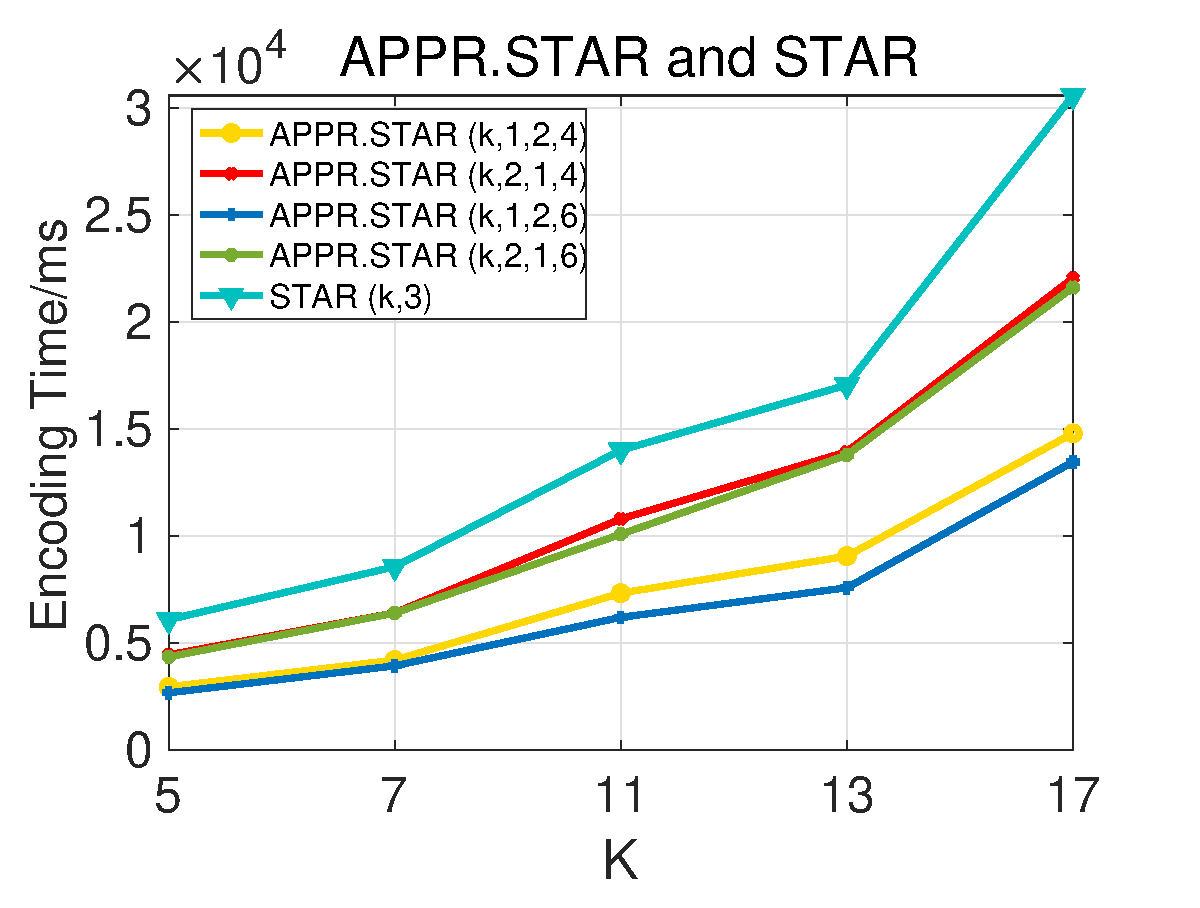
\includegraphics[width = 0.23\linewidth]{photo/experiment/Encoding-Star.eps}
}
\subfigure[APPR.TIP and TIP]{
    \label{fig-encodingTIP}
    \includegraphics[width = 0.23\linewidth]{photo/experiment/Encoding-TIP.eps}
}
\subfigure[APPR.TIP/STAR and RS]{
    \label{fig-encodingRS}
    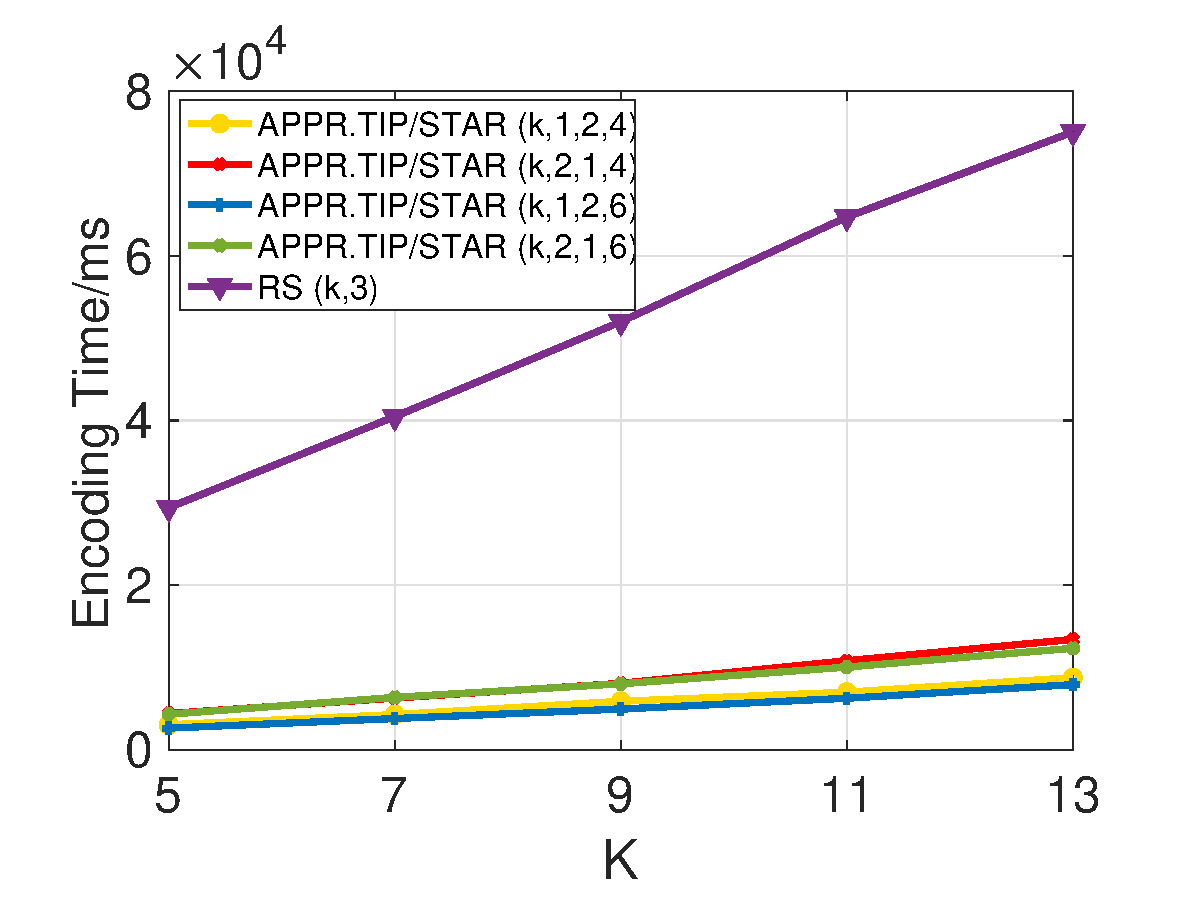
\includegraphics[width = 0.23\linewidth]{photo/experiment/Encoding-RS.eps}
}
\subfigure[APPR.TIP/STAR and LRC]{
    \label{fig-encodingLRC}
    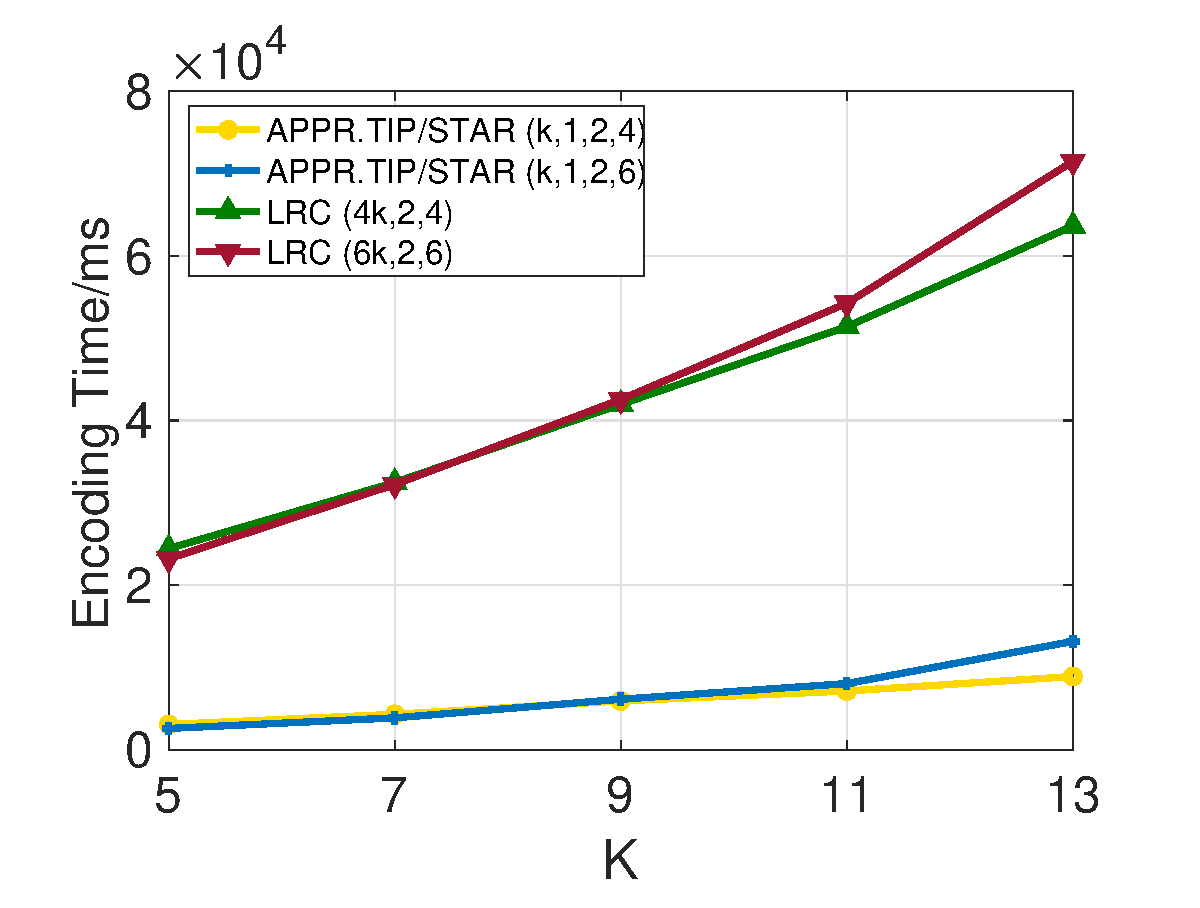
\includegraphics[width = 0.23\linewidth]{photo/experiment/Encoding-LRC.eps}
}\vspace{-0.5cm}
\caption{Encoding Time Comparison between AP method and other method}\label{fig-encoding}
\end{figure*}


\begin{figure*}[ht]
\subfigure{
    \label{fig-decoding-1-STAR}
    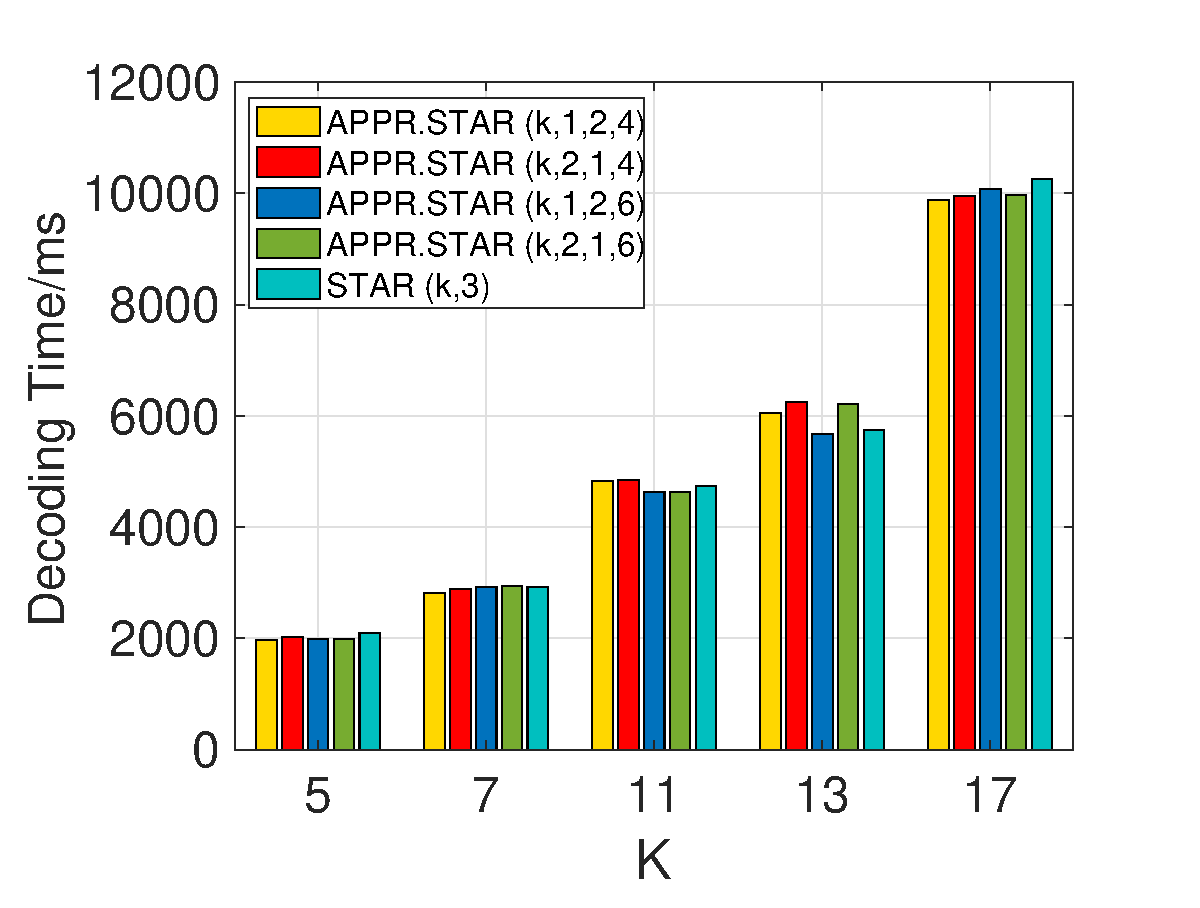
\includegraphics[width = 0.23\linewidth]{photo/experiment/Decoding-1-Star.eps}
}
\subfigure{
    \label{fig-decoding-1-TIP}
    \includegraphics[width = 0.23\linewidth]{photo/experiment/Decoding-1-TIP.eps}
}
\subfigure{
    \label{fig-decoding-1-RS}
    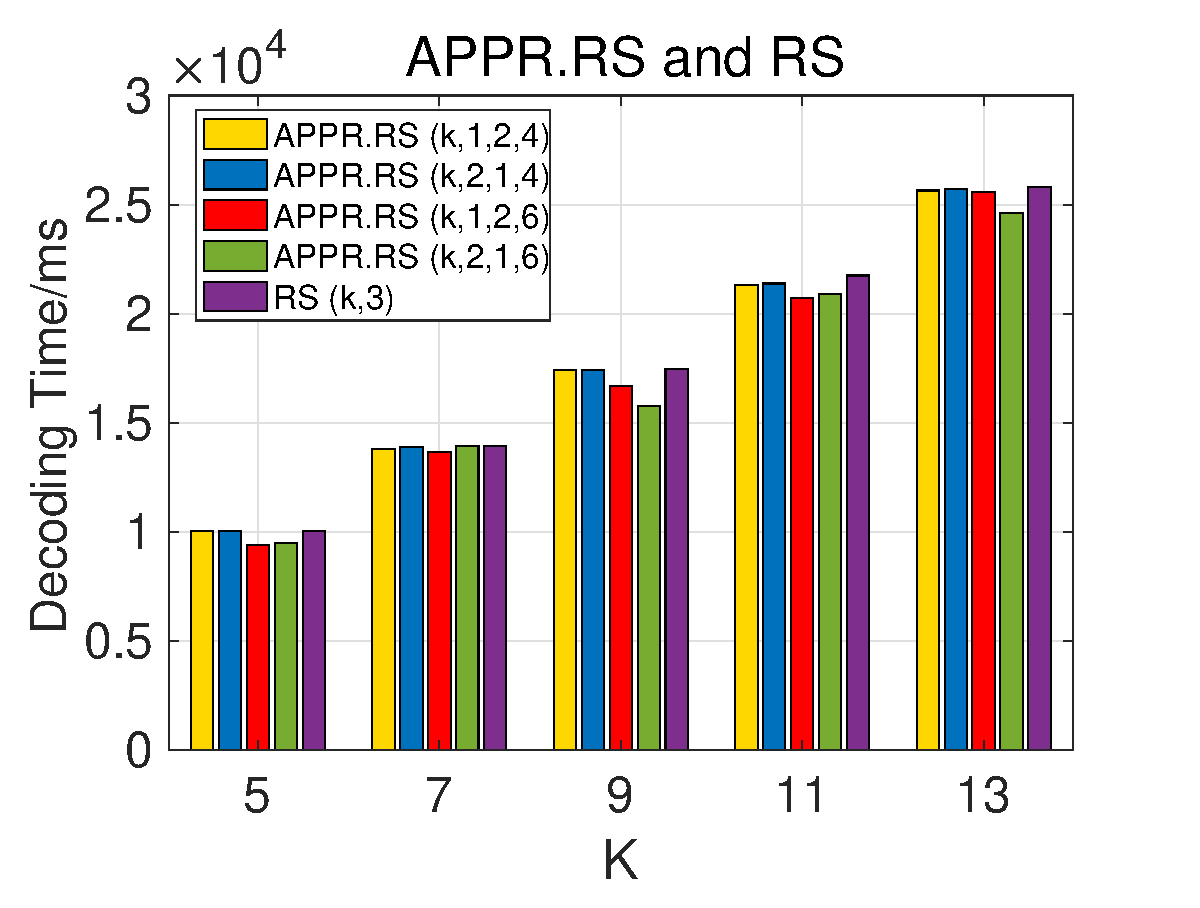
\includegraphics[width = 0.23\linewidth]{photo/experiment/Decoding-1-RS.eps}
}
\subfigure{
    \label{fig-decoding-1-LRC}
    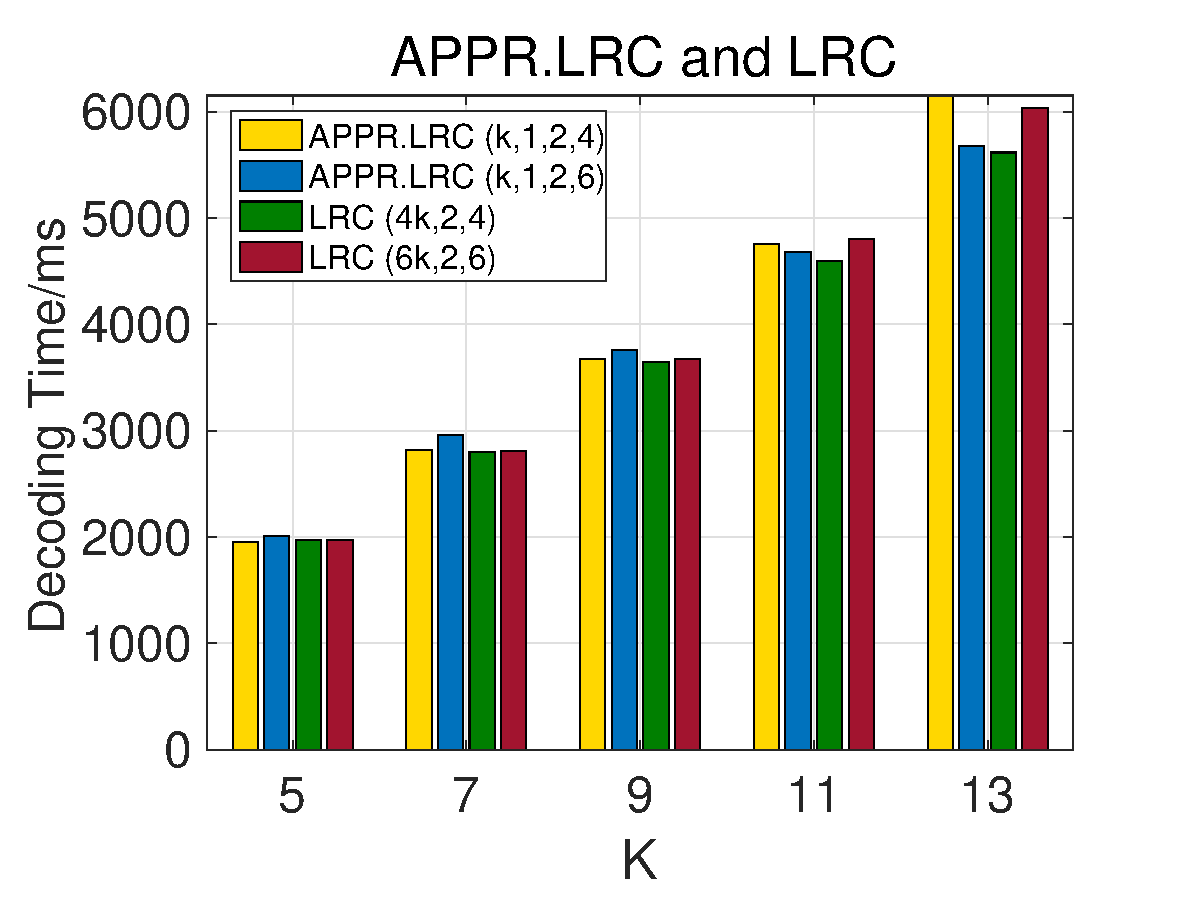
\includegraphics[width = 0.23\linewidth]{photo/experiment/Decoding-1-LRC.eps}
}\vspace{-0.5cm}
\caption{Decoding Time Comparison in One Disk between AP method and other method}\label{fig-decoding-1}
\end{figure*}


\begin{figure*}[ht]
\subfigure{
    \label{fig-decoding-2-STAR}
    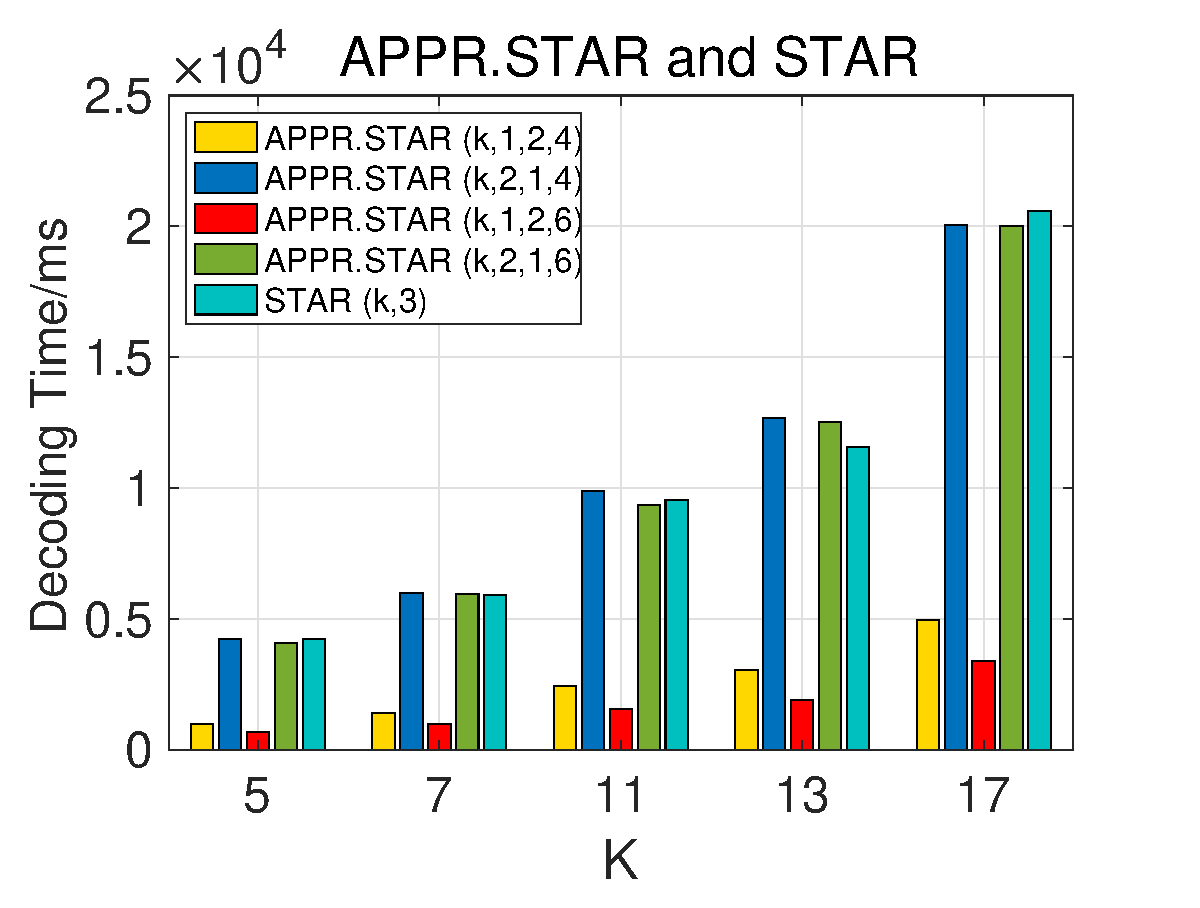
\includegraphics[width = 0.23\linewidth]{photo/experiment/Decoding-2-Star.eps}
}
\subfigure{
    \label{fig-decoding-2-TIP}
    \includegraphics[width = 0.23\linewidth]{photo/experiment/Decoding-2-TIP.eps}
}
\subfigure{
    \label{fig-decoding-2-RS}
    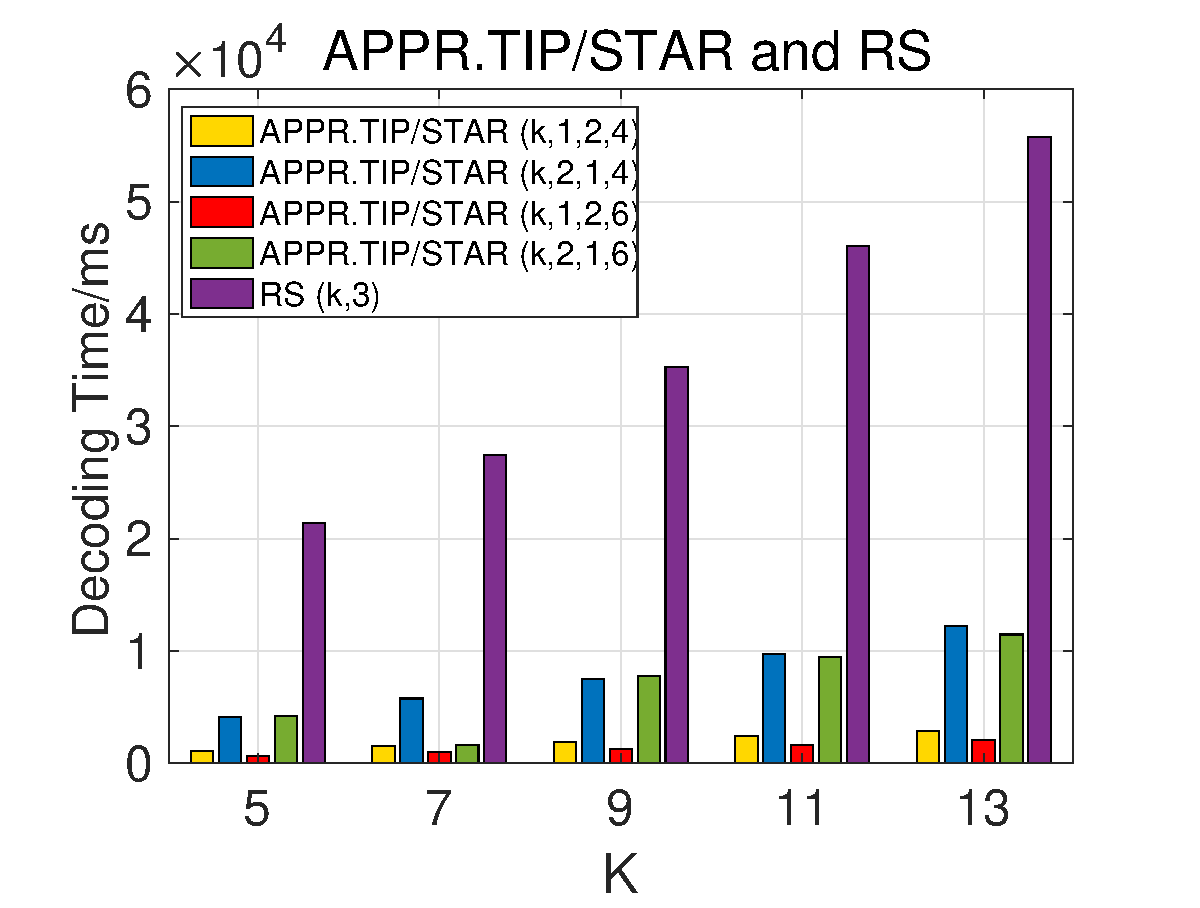
\includegraphics[width = 0.23\linewidth]{photo/experiment/Decoding-2-RS.eps}
}
\subfigure{
    \label{fig-decoding-2-LRC}
    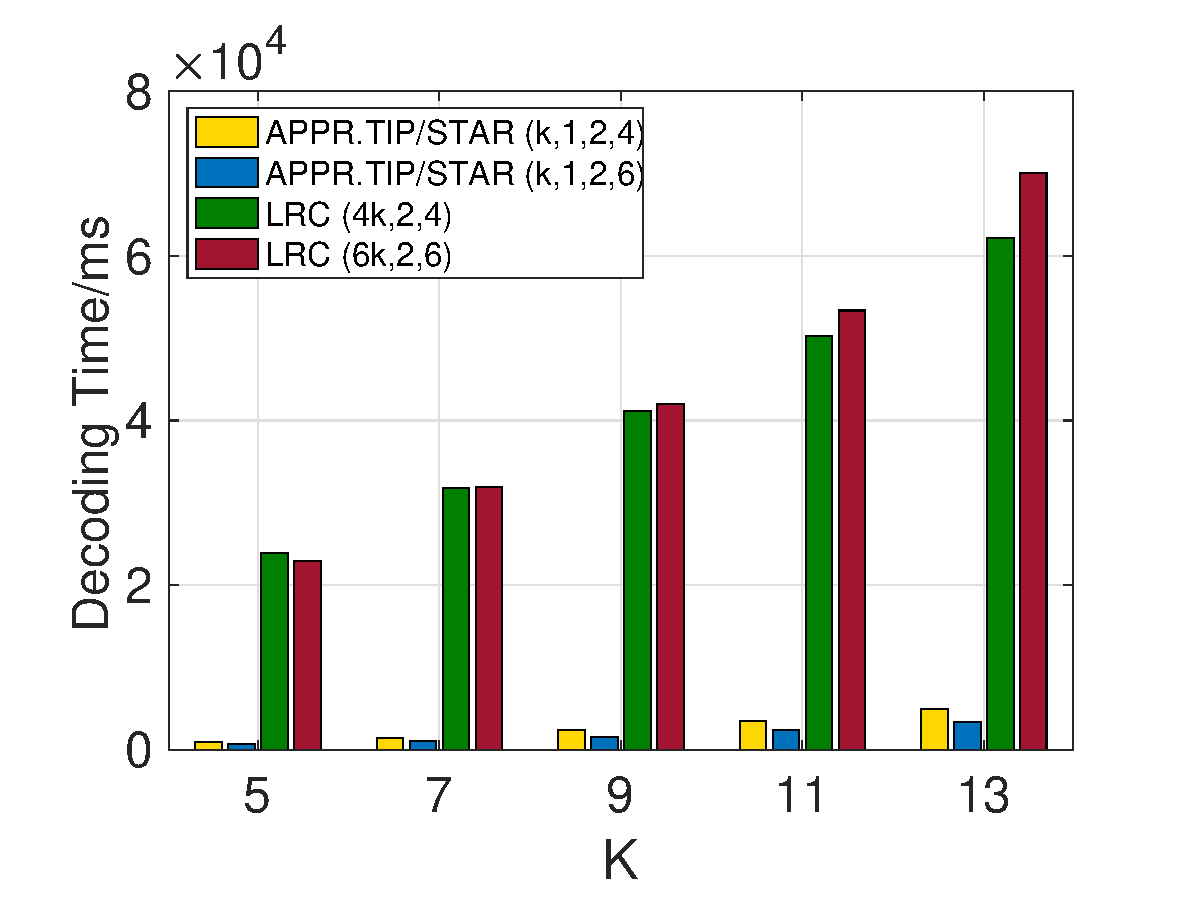
\includegraphics[width = 0.23\linewidth]{photo/experiment/Decoding-2-LRC.eps}
}\vspace{-0.5cm}
\caption{Decoding Time Comparison in Two Disk between AP method and other method}\label{fig-decoding-2}
\end{figure*}

\begin{figure*}[ht]
\subfigure{
    \label{fig-decoding-3-STAR}
    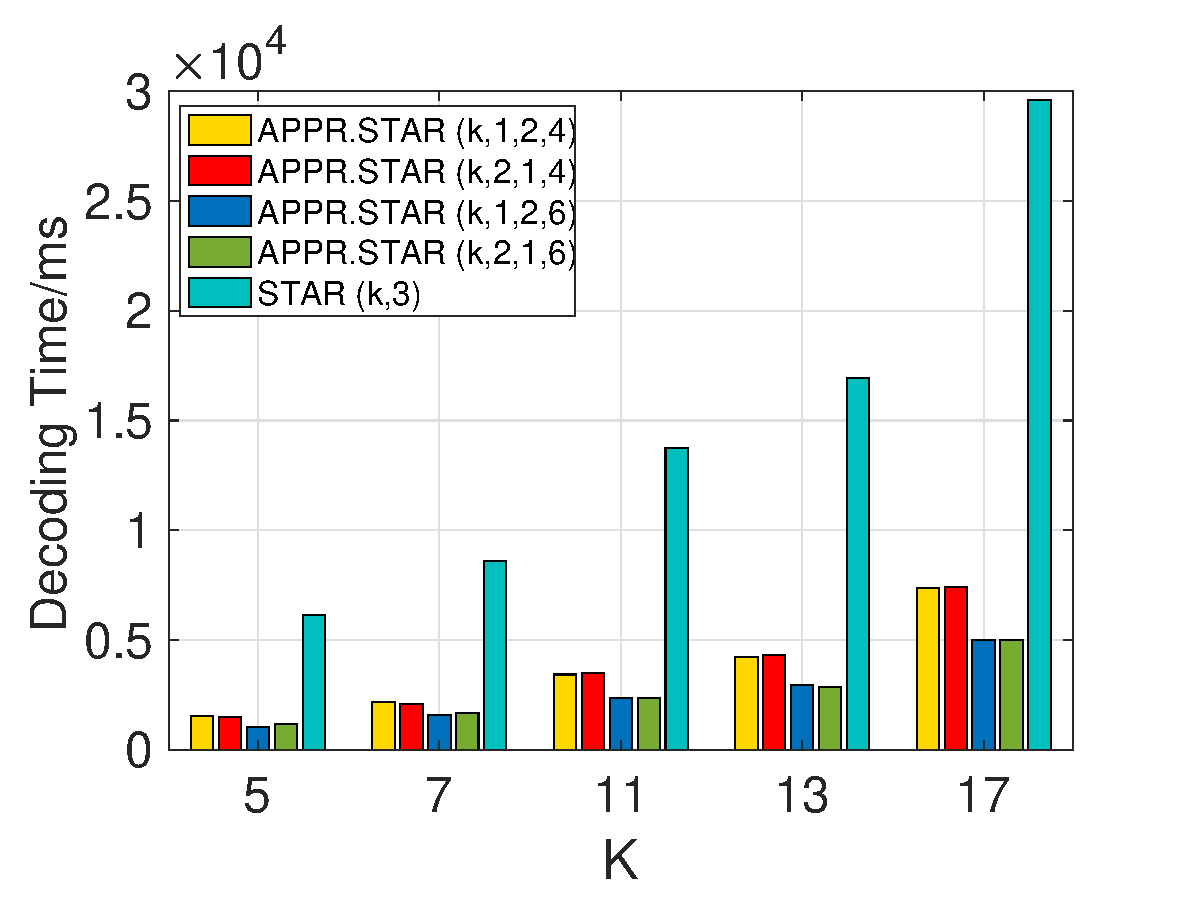
\includegraphics[width = 0.23\linewidth]{photo/experiment/Decoding-3-Star.eps}
}
\subfigure{
    \label{fig-decoding-3-TIP}
    \includegraphics[width = 0.23\linewidth]{photo/experiment/Decoding-3-TIP.eps}
}
\subfigure{
    \label{fig-decoding-3-RS}
    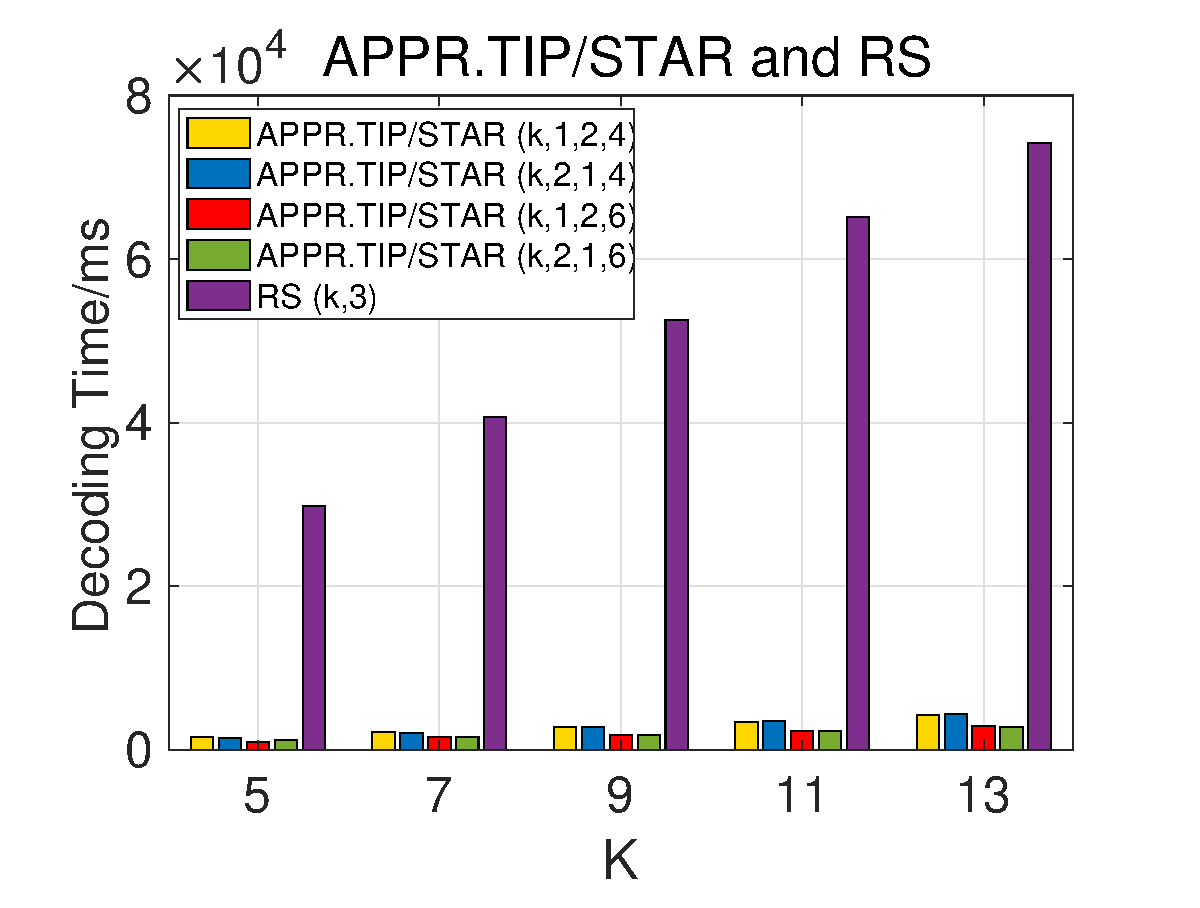
\includegraphics[width = 0.23\linewidth]{photo/experiment/Decoding-3-RS.eps}
}
\subfigure{
    \label{fig-decoding-3-LRC}
    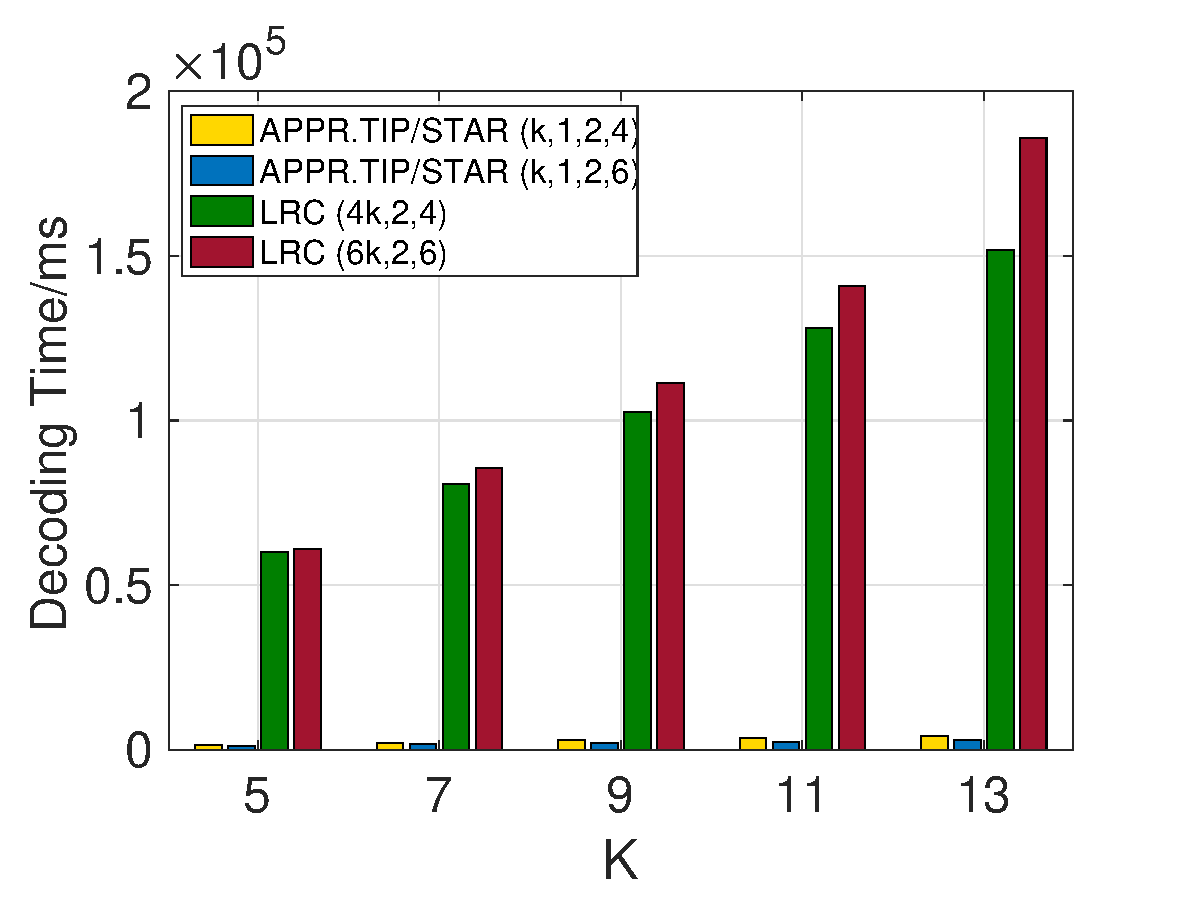
\includegraphics[width = 0.23\linewidth]{photo/experiment/Decoding-3-LRC.eps}
}\vspace{-0.5cm}
\caption{Decoding Time Comparison in Two Disk between AP method and other method}\label{fig-decoding-3}
\end{figure*}

\subsubsection{Decoding Time under One Failure Node Condition Analysis}

In this section, we compared the decoding time of Approximate Code with TIP code, Star code, RS code and LRC codes under single failure node condition, respectively. $k$ changes from 5 to 17.
\begin{itemize}
    \item APPR.STAR ($k,1,2,4$), APPR.STAR ($k,2,1,4$), APPR.STAR ($k,1,2,6$), APPR.STAR ($k,2,1,6$) and STAR ($k,3$): Figure \ref{fig-decoding-1-STAR} illustrates that the decoding time of Approximate Code is almost the same as STAR code when sinlge node fails and the rate of optimization is up to 5.4\% (between APPR.STAR ($k,1,2,4$) and STAR ($k,3$) when $k = 5$).
    \item APPR.STAR ($k,1,2,4$), APPR.STAR ($k,2,1,4$), APPR.STAR ($k,1,2,6$), APPR.STAR ($k,2,1,6$) and TIP($k,3$): Figure \ref{fig-decoding-1-TIP} illustrates that the decoding time of Approximate Code is almost the same as TIP code when sinlge node fails and the rate of optimization is up to 8.8\% (between APPR.TIP($k,1,2,4$) and TIP($k,3$) when k = 17).
    \item APPR.STAR ($k,1,2,4$), APPR.STAR ($k,2,1,4$), APPR.STAR ($k,1,2,6$), APPR.STAR ($k,2,1,6$) and RS($k,3$): From the Figure \ref{fig-decoding-1-RS}, we could find out that the Approximate Code decodes largely faster than RS code. The rate of optimization is up to 80.2\% (between APPR.TIP/STAR ($k,1,2,4$) and RS($k,3$) when $k = 5$).
    \item APPR.TIP/STAR ($k,1,2,4$), APPR. TIP/STAR ($k,2,1,4$), APPR. TIP/STAR ($k,1,2,6$), APPR. TIP/STAR ($k,2,1,6$) and LRC ($k,4,3$), LRC  ($k,6,3$):  According to Figure \ref{fig-decoding-1-LRC}, we could see that Approximate Code and LRC codes have no big gap when encoding one lost node. The rate of optimization is up to $5.8\%$ (between APPR.TIP/STAR ($k,1,2,6$) and LRC ($k, 6, 2$) when $k = 13$).
\end{itemize}

We combined the decoding time of five codes under one failure node condition in Figure \ref{fig-decoding-1-combine} with $k=5$. The results show that RS code has the worst one node decoding performance among five codes and the performance of other four codes are almost the same. The main reason is that XOR-based codes have lower computational overhead than RS-based codes.\par

\begin{figure*}[ht]
\subfigure[Encoding Time]{
    \label{fig-encoding-combine}
    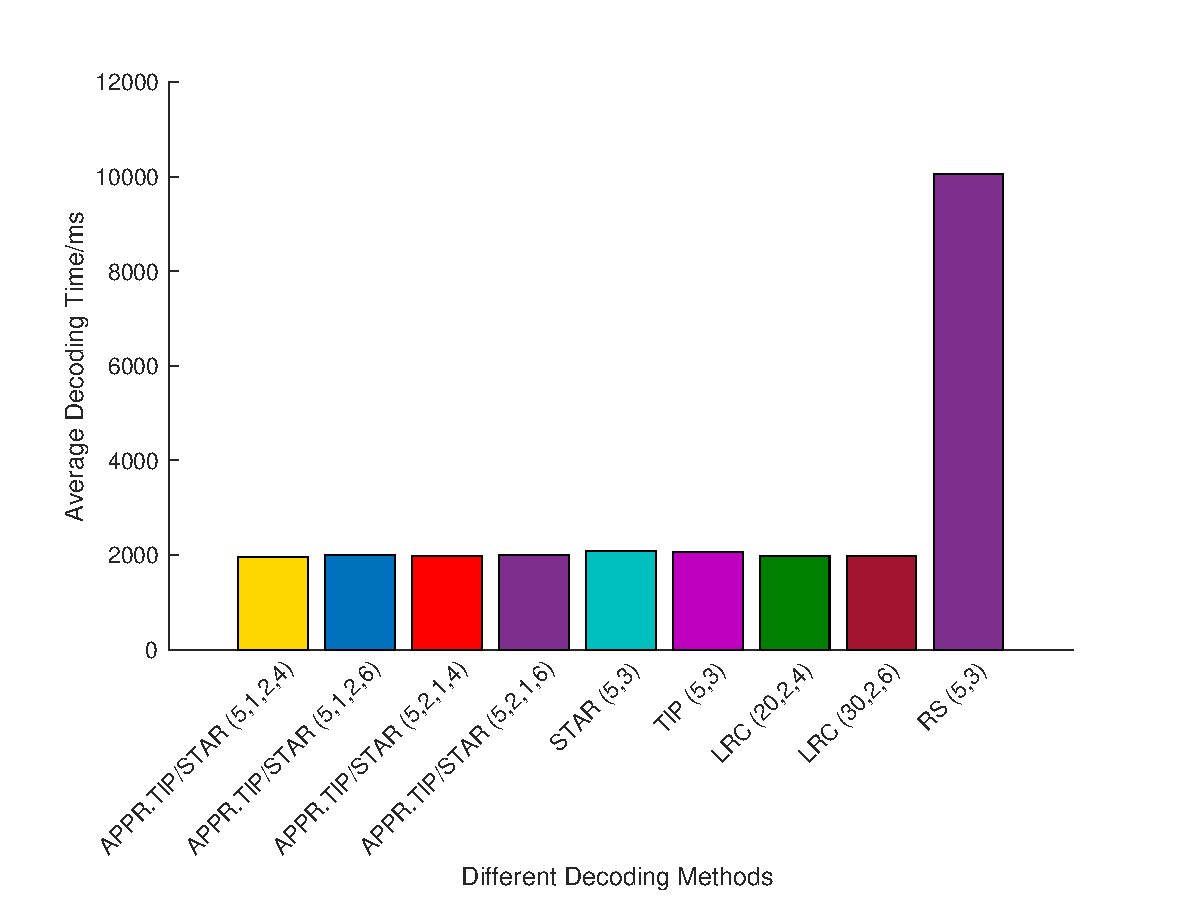
\includegraphics[width = 0.23\linewidth]{photo/experiment/Bar-Encoding.eps}
}
\subfigure[Decoding Time in One Node Failure]{
    \label{fig-decoding-1-combine}
    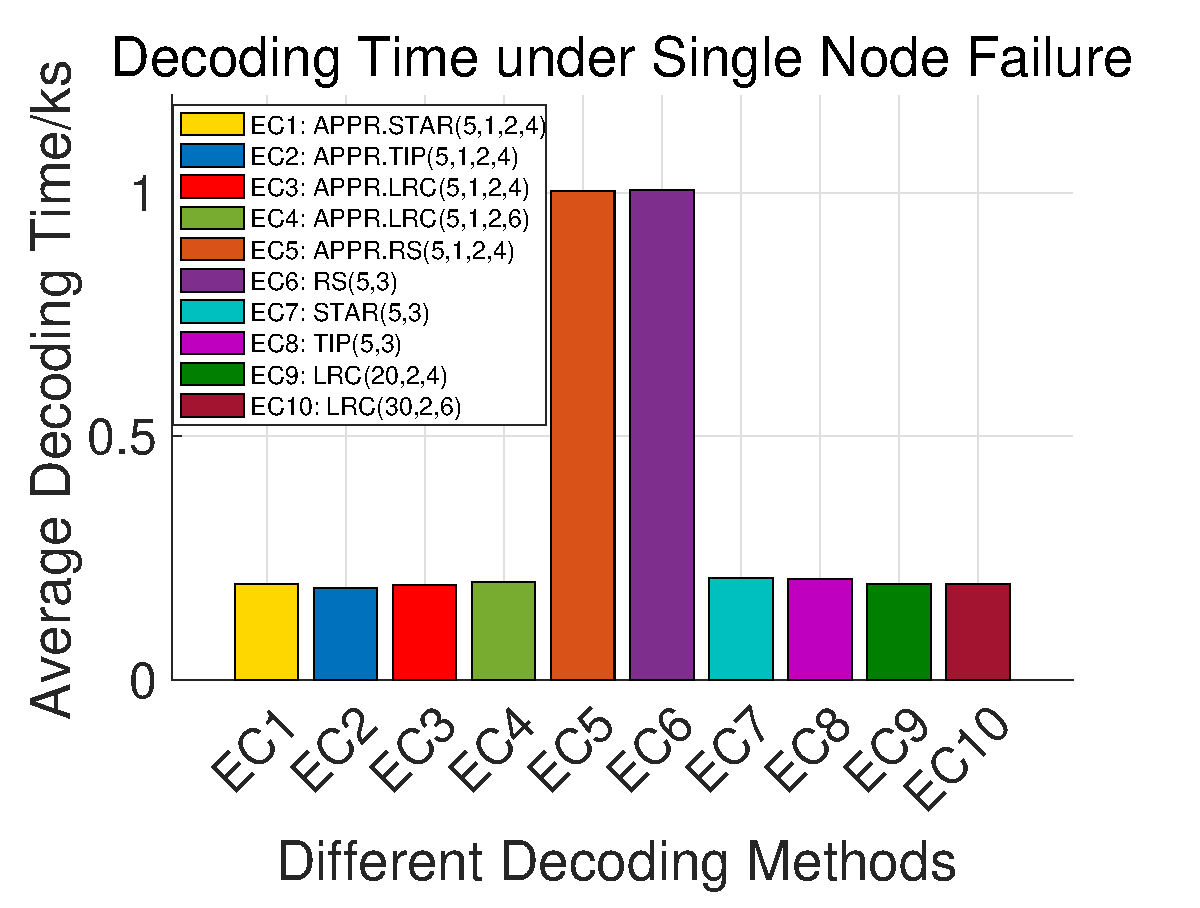
\includegraphics[width = 0.23\linewidth]{photo/experiment/Bar-Decoding-1.eps}
}
\subfigure[Decoding Time in Two Node Failure]{
    \label{fig-decoding-2-combine}
    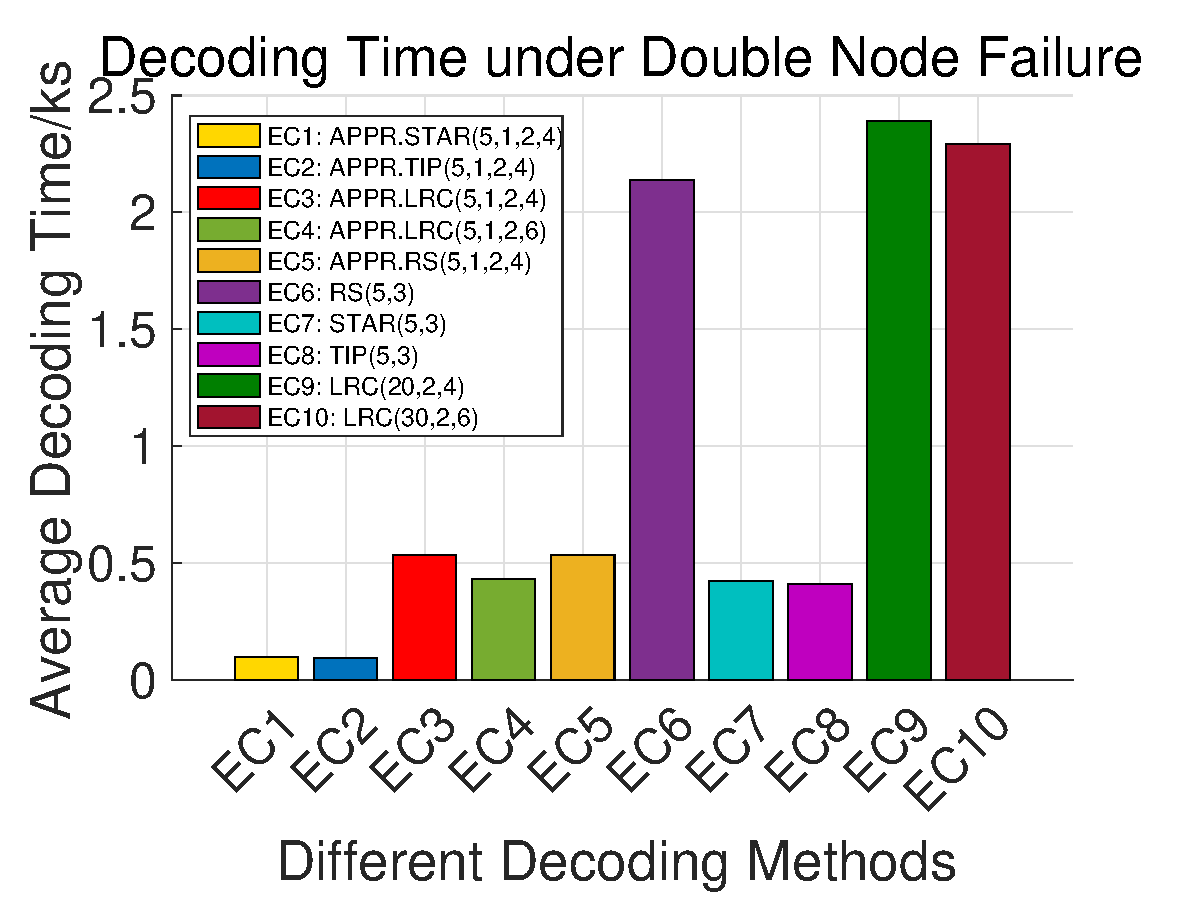
\includegraphics[width = 0.23\linewidth]{photo/experiment/Bar-Decoding-2.eps}
}
\subfigure[Decoding Time in Three Node Failure]{
    \label{fig-decoding-3-combine}
    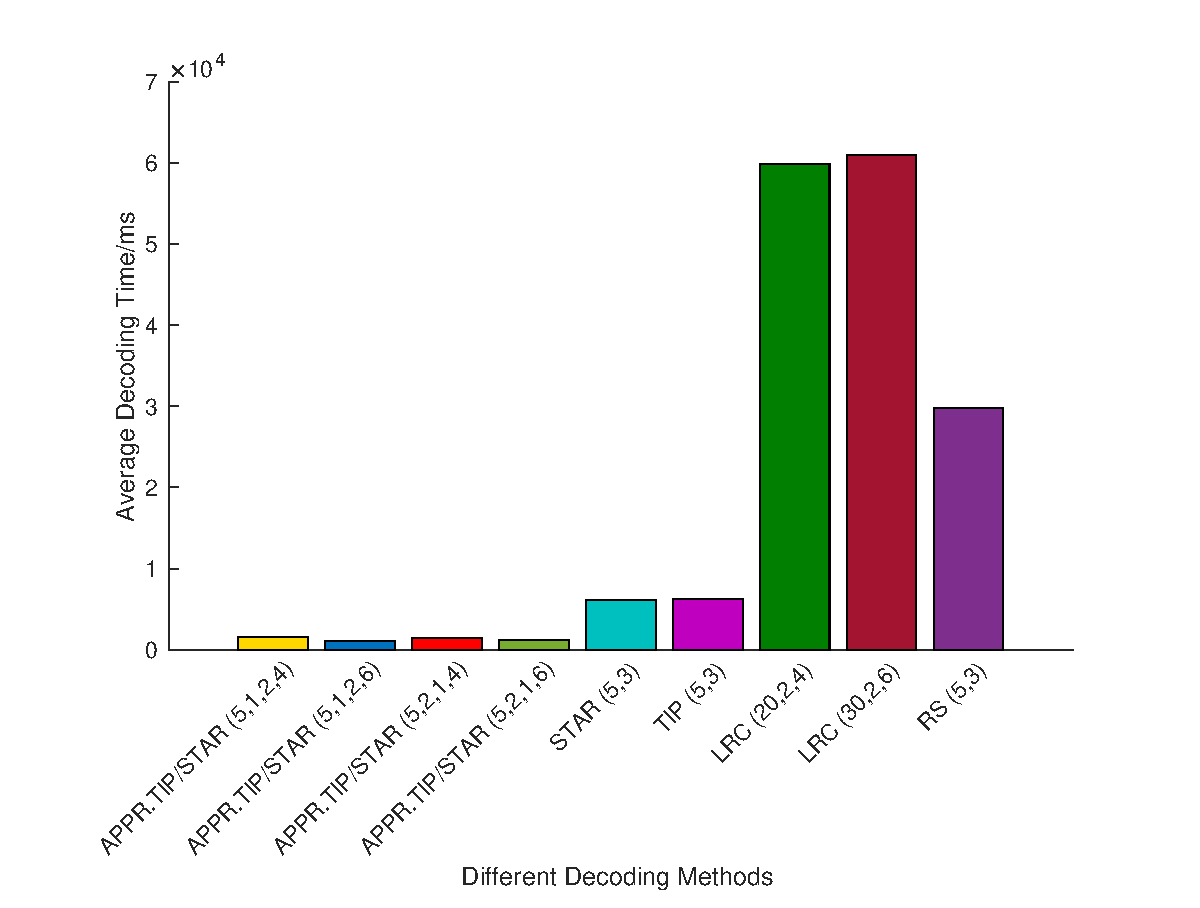
\includegraphics[width = 0.23\linewidth]{photo/experiment/Bar-Decoding-3.eps}
}
\caption{Comparison of several matrics between different methods when number of data nodes are 5}\label{fig-BAR}
\end{figure*}


\subsubsection{Decoding Time under Two Failure Nodes Condition Analysis}
In this part, we compared the decoding time of Approximate Code with TIP code, Star code, RS code and LRC codes under two failure nodes condition, respectively. $k$ changes from 5 to 17.
\begin{itemize}
    \item APPR.STAR ($k,1,2,4$), APPR.STAR ($k,2,1,4$), APPR.STAR ($k,1,2,6$), APPR.STAR ($k,2,1,6$) and STAR ($k,3$): Figure \ref{fig-decoding-2-STAR} illustrates that the rate of optimization is up to $83.9\%$ (between APPR.STAR ($k,1,2,6$) and STAR ($k,3$) when $k = 5$).
    \item APPR.STAR ($k,1,2,4$), APPR.STAR ($k,2,1,4$),  APPR.STAR ($k,1,2,6$), APPR.STAR ($k,2,1,6$) and TIP($k,3$): This condition is similar to STAR code. Figure \ref{fig-decoding-2-TIP} illustrates that the rate of optimization is up to $84.8\% $(between APPR.TIP($k,1,2,6$) and TIP($k,3$) when $k = 9$).
    \item APPR.STAR ($k,1,2,4$), APPR.STAR ($k,2,1,4$),  APPR.STAR ($k,1,2,6$), APPR.STAR ($k,2,1,6$) and RS($k,3$): From the Figure \ref{fig-decoding-2-RS}, we could find out that the Approximate Code decodes largely faster than RS code under two failure nodes condition. The rate of optimization is up to $96.9\%$ (between APPR.TIP/STAR ($k,1,2,6$) and RS($k,3$) when $k = 5$).
    \item APPR.TIP/STAR ($k,1,2,4$), APPR. TIP/STAR ($k,2,1,4$),  APPR. TIP/STAR ($k,1,2,6$), APPR. TIP/STAR ($k,2,1,6$) and LRC ($k,4,3$), LRC ($k,6,3$):
    According to Figure \ref{fig-decoding-2-LRC}, we could see that Approximate Code largely reduces the decoding time when two nodes fail, compared with LRC codes. The rate of optimization is up to $97.2\%$ (between APPR.TIP/STAR ($k,1,2,6$) and LRC ($k, 6, 2$) when $k = 5$).
\end{itemize}

The combined decoding time of five codes under two failure node condition are shown in Figure \ref{fig-decoding-2-combine} ($k=5$). The results show that RS code and LRC codes has the worst two failure nodes decoding performance while APPR.TIP/STAR ($k,1,2,6$) and APPR.TIP/STAR ($k,1,2,4$) perform best among all kinds of codes. The main reasons are that: On two failure nodes condition, RS code and LRC codes decode data based on RS method which have heavy computational cost while APPR.TIP/STAR ($k,1,2,6$) and APPR.TIP/STAR ($k,1,2,4$) do the approximate recovery which means they only recover important data at this time.

\subsubsection{Decoding Time under Three Failure Nodes Condition Analysis}
In this part, we compared the decoding time of Approximate Code with TIP code, Star code, RS code and LRC codes under three failure nodes condition, respectively. $k$ changes from 5 to 17.
\begin{itemize}
    \item APPR.STAR ($k,1,2,4$), APPR.STAR ($k,2,1,4$), APPR.STAR ($k,1,2,6$), APPR.STAR ($k,2,1,6$) and STAR ($k,3$): Figure \ref{fig-decoding-3-STAR} illustrates that the rate of optimization is up to $83.5\%$ (between APPR.STAR ($k,1,2,6$) and STAR ($k,3$) when $k = 5$).
    \item APPR.STAR ($k,1,2,4$), APPR.STAR ($k,2,1,4$), APPR.STAR ($k,1,2,6$), APPR.STAR ($k,2,1,6$) and TIP($k,3$): This condition is similar to STAR code. Figure \ref{fig-decoding-3-TIP} illustrates that the rate of optimization is up to 82.2\% (between APPR.TIP($k,1,2,6$) and TIP($k,3$) when $k = 5$).
    \item APPR.STAR ($k,1,2,4$), APPR.STAR ($k,2,1,4$), APPR.STAR ($k,1,2,6$), APPR.STAR ($k,2,1,6$) and RS($k,3$): From the Figure \ref{fig-decoding-3-RS}, we could find out that the Approximate Code decodes largely faster than RS code under three failure nodes condition. The rate of optimization is up to $96.7\%$ (between APPR.TIP/STAR ($k,1,2,6$) and RS($k,3$) when $k = 5$).
    \item APPR.TIP/STAR ($k,1,2,4$), APPR. TIP/STAR ($k,2,1,4$), APPR. TIP/STAR ($k,1,2,6$), APPR. TIP/STAR ($k,2,1,6$)  \\
    and LRC($k,4,3$), LRC ($k,6,3$):
    According to Figure \ref{fig-decoding-3-LRC}, we could see that Approximate Code largely reduces the decoding time when three nodes fail, compared with LRC codes. The rate of optimization is up to $98.3\%$  (between APPR.TIP/STAR ($k,1,2,6$) and LRC ($k, 6, 2$) when $k = 5$).
\end{itemize}

\iffalse
\begin{figure}[ht]
\centering
\subfigure[]{
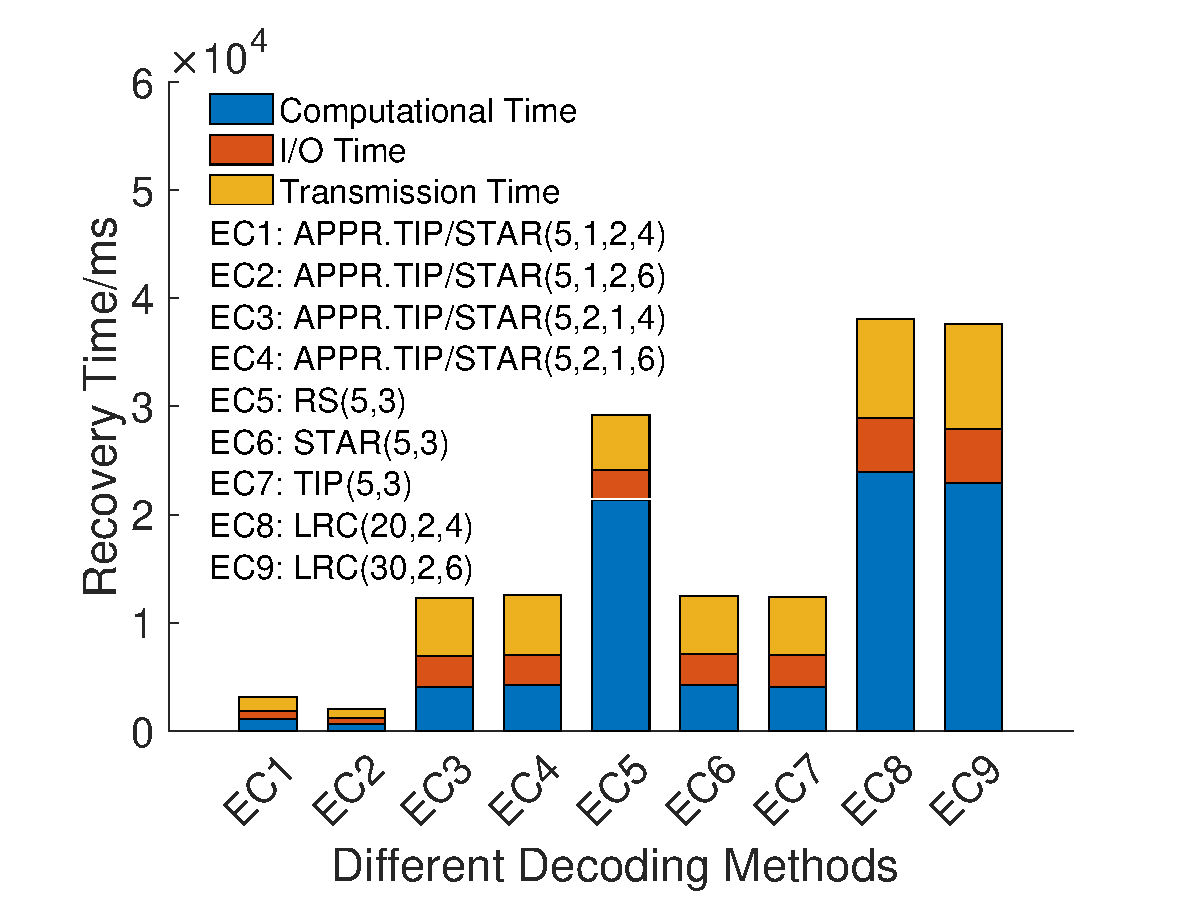
\includegraphics[width=0.5\linewidth]{photo/experiment/Recovery-2.eps}\label{fig-rec-2}
}\hspace{-0.4cm}
\subfigure[]{
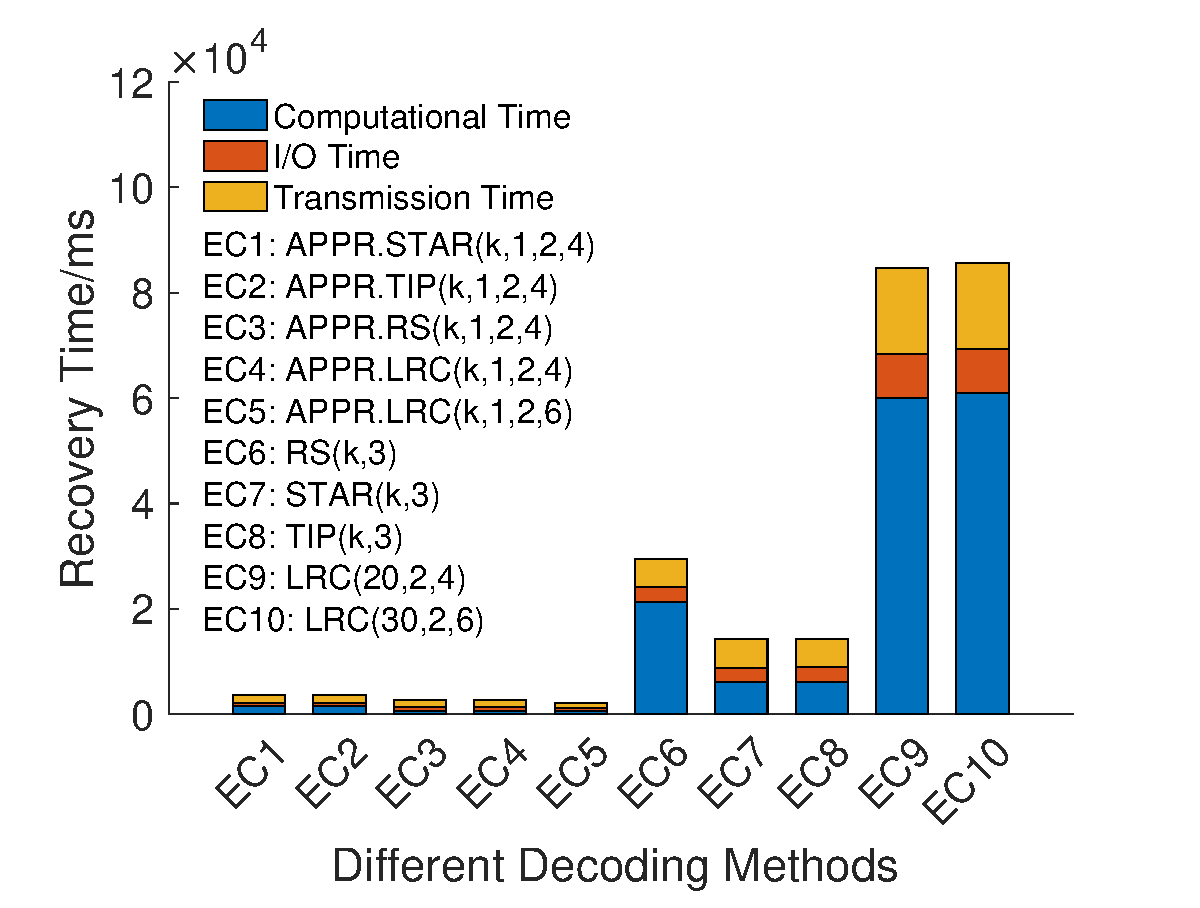
\includegraphics[width=0.5\linewidth]{photo/experiment/Recovery-3.eps}\label{fig-rec-3}
}
\caption{Recovery time Result using Frame Interpolation}
\label{fig-recoverytime}
\end{figure}
\fi

\begin{figure}[ht]
\centering
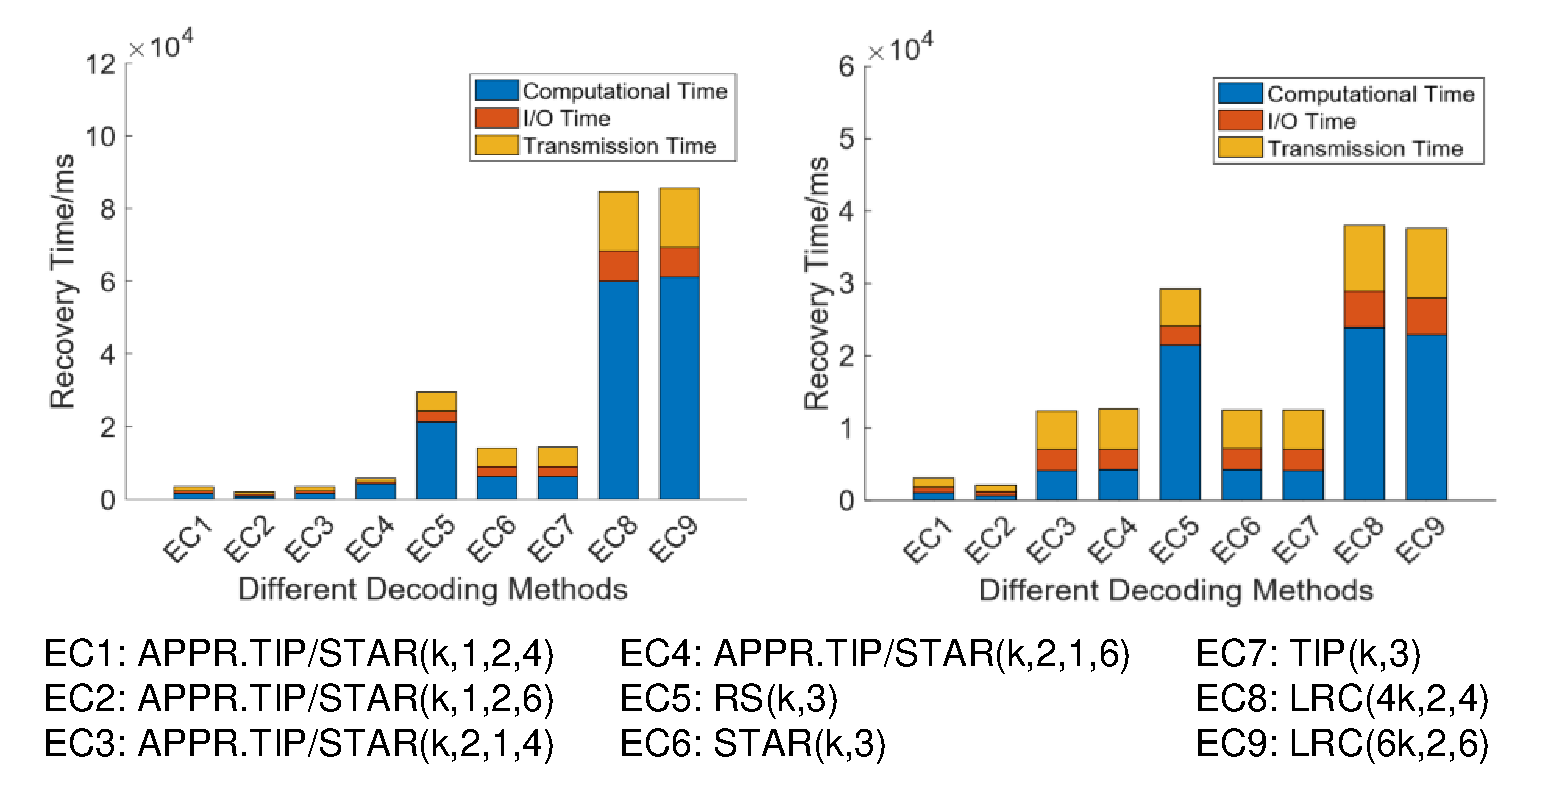
\includegraphics[width=\linewidth]{photo/experiment/Recovery-2-3.pdf}\label{fig-rec-3}
\caption{Recovery time Result using Frame Interpolation}
\label{fig-recoverytime}
\end{figure}

The combined decoding time of five codes under three failure node condition are shown in Figure \ref{fig-decoding-3-combine} ($k$=5). The results show that LRC has the worst three failure nodes decoding performance. The main reasons are that: On three failure nodes condition, LRC codes decode data through the global parities which has a longer parity chain. For example $LRC (44,4,2)$ use 44 nodes to recover the three lost nodes. the computational cost of GF operations is also larger than XOR operations. On the other hand, All kinds of Approximate Code perform best among all kinds of codes because they only recover important data at this time.


\subsection{Frame Recovery}
Here we present the frame recovery result by using frame interpolation \cite{meyer2015phase, niklaus2018context,van2017frame}. As shown in Figure\ref{fig-frameRecovery}, The top 3 figures are the original frames. When frame 2 lost, the interpolation techniques can output \ref{fig-recoverof2} by the input of \ref{fig-interop1} and \ref{fig-interop3}. The recovered frame has a lower resolution and may differ from the original image, but since the unconstrained frame contains most of the context information, the video is still available, which validates the fact that the video can tolerate a certain amount of data loss.



\begin{figure}[ht]
\centering
\subfigure[Frame 1]{

\includegraphics[width=0.3\linewidth]{photo/Frame/1.jpg}\label{fig-interop1}
}
\subfigure[Frame 2]{
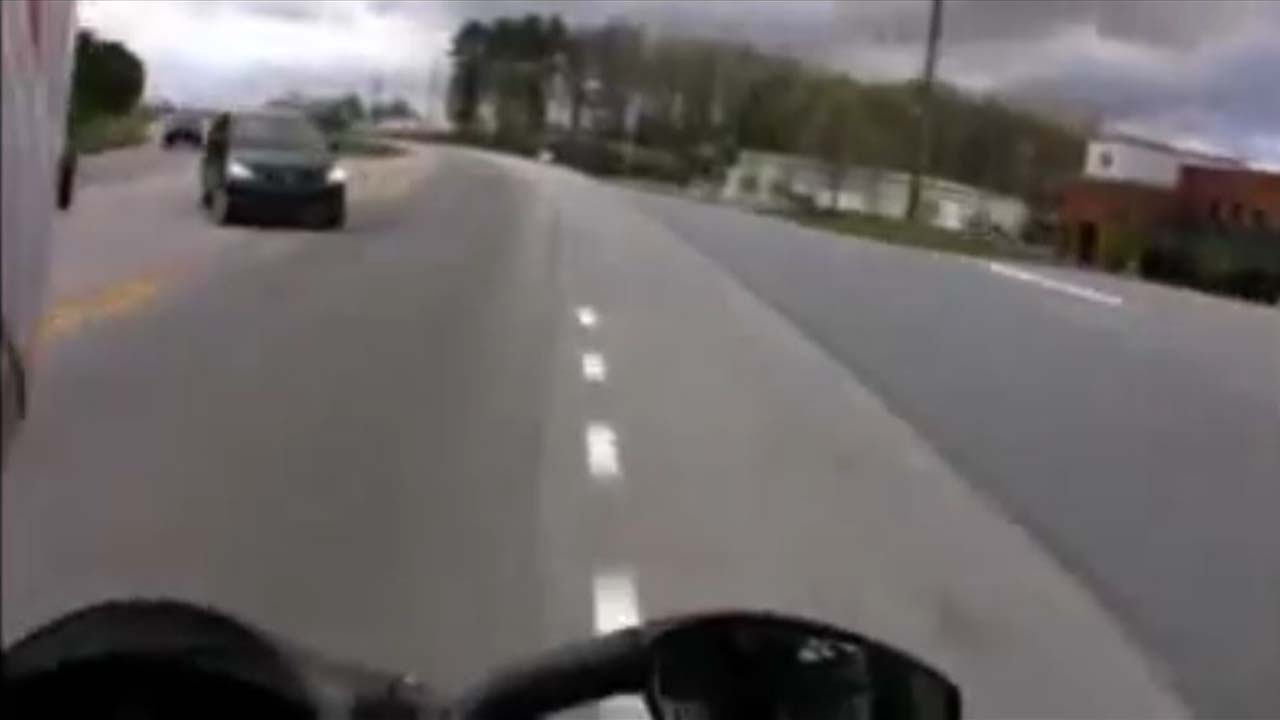
\includegraphics[width=0.3\linewidth]{photo/Frame/2.jpg}\label{fig-interop2}
}
\subfigure[Frame 3]{

\includegraphics[width=0.3\linewidth]{photo/Frame/3.jpg}\label{fig-interop3}
}

\subfigure[Recovery of Frame 2]{

\includegraphics[width=0.5\linewidth]{photo/Frame/2_1.jpg}\label{fig-recoverof2}
}
\caption{Frame Recovery Result using Frame Interpolation}
\label{fig-frameRecovery}
\end{figure}

\section{Conclusion}\label{Conclusion}
In this paper, we present the Approximate Code, which is the framework for video tiered storage in cloud systems. The Approximate Code can segment the input erasure codes and provide different fault tolerance for data of different importance. For important data, the Approximate Code provides 3DFTs, and for non-critical data, the Approximate Code provides single or double parity, thus saving storage costs and speeding up recovery, while having good update write performance. We conducted several experiments in the Hadoop system and found that compared to traditional 3DFTs using various erasure codes such as RS, STAR and TIP-Code, Approximate Code reduces the number of parities by up to 55\%, saves the storage cost by up to 20.8\%, increase the recovery speed by up to 1.25X when single disk fails, and can reconstruct the whole video data via fuzzification when triple disks fail.

\bibliographystyle{ACM-Reference-Format}
\bibliography{ApproximateCode}

\end{document}
